%% add 'handout' option for handouts, and pgfpages for 2-on-1
%\documentclass[smaller,compress]{beamer}   
\documentclass[compress]{beamer}   
%\usepackage{pgfpages}
%\pgfpagesuselayout{2 on 1}[letterpaper,border shrink=5mm]
%\pgfpagesuselayout{4 on 1}[letterpaper,border shrink=5mm]
%\pgfpagesuselayout{2 on 1}[a4,border shrink=5mm]
\usepackage{color}
\usepackage{alltt}
\usepackage[latin1]{inputenc}

../rinfinance2010/highlight.sty



\mode<presentation>
{
  %\usetheme[secheader]{Madrid} % nice (once my coloroverrides are sorted out)
  %\usetheme{AnnArbor}	% nice!	
  %\usetheme{Malmoe}	% nice!	
  \usetheme{Warsaw}	% nice!	

  %\usetheme[secheader]{Boadilla} % ok
  %\usecolortheme{whale}
  %\usecolortheme{orchid}
}

% Delete this, if you do not want the table of contents to pop up at
% the beginning of each subsection (or section)
% edd: Does not work in handout mode, and we have too many section/subsections
\AtBeginSection[]{%
  \begin{frame}<beamer>%
    %\tiny
    \frametitle{Outline}%
    \tableofcontents[currentsection]
  \end{frame}
}


% If you wish to uncover everything in a step-wise fashion, uncomment the following command: 
%\beamerdefaultoverlayspecification{<+->}

\newcommand{\MedSkip}{\medskip \par} % add \pause if desired 
\newcommand{\SmallSkip}{\smallskip} % add \pause if desired 

\usepackage[english]{babel}   	% or whatever
\usepackage[latin1]{inputenc}	% or whatever
\usepackage{times}
\usepackage[T1]{fontenc}		% Or whatever. Note that the encoding and the 
								% font should match. If T1 does not look
                                % nice, try deleting the line with the fontenc.
\usepackage{highlight}
\usepackage{color}
\usepackage{alltt}

% \usepackage{animate}

\usepackage{listings}
\lstset{ %
  language=R,                   % choose the language of the code
  basicstyle=\scriptsize,       % the size of the fonts that are used for the code
  numbers=left,                 % where to put the line-numbers
  numberstyle=\tiny,            % the size of the fonts that are used for the line-numbers
  stepnumber=1,                 % the step between two line-numbers. If it's 1 each line will be numbered
  numbersep=5pt,                % how far the line-numbers are from the code
  backgroundcolor=\color{white},% choose the background color. You must add \usepackage{color}
  showspaces=false,             % show spaces adding particular underscores
  showstringspaces=false,       % underline spaces within strings
  showtabs=false,               % show tabs within strings adding particular underscores
  frame=single,                 % adds a frame around the code
  tabsize=2,                    % sets default tabsize to 2 spaces
  captionpos=b,                 % sets the caption-position to bottom
  breaklines=true,              % sets automatic line breaking
  breakatwhitespace=false,      % sets if automatic breaks should only happen at whitespace
  escapeinside={\%*}{*)}        % if you want to add a comment within your code
}

\hypersetup{                  		% beamer colors taken from elsewhere
  hyperindex,%				% works with the beetle colour scheme
  colorlinks,%
  linktocpage,%
  plainpages=true,%
  linkcolor=myOrange,%
  citecolor=myDarkGrey,%
  urlcolor=myDarkBlue,%
  pdfstartview=Fit,%
  pdfview={XYZ null null null}%
}
%\hypersetup{                  		% beamer colors taken from elsewhere
%  hyperindex,%				% works with the beetle colour scheme
%  colorlinks%
%  linktocpage,%
%  plainpages=false,%
%  linkcolor=eddBlue,%
%  citecolor=eddDarkGrey,%
%  urlcolor=eddDarkBlue,%
%  pdfstartview=Fit,%
%  pdfview={XYZ null null null}%
%}

\RequirePackage{color}
\definecolor{Red}{rgb}{0.7,0,0}
\definecolor{myOrange}{rgb}{0.8,0.5,0.0}
\definecolor{myBlue}{rgb}{0.0,0.0,0.4}
\definecolor{myDarkBlue}{rgb}{0.1,0.1,0.4}
\definecolor{myDarkGrey}{rgb}{0.15,0.15,0.15}
% Doug's
\definecolor{Sinput}{rgb}{0,0,0.56}
\definecolor{Scode}{rgb}{0,0,0.56}
\definecolor{Soutput}{rgb}{0.56,0,0}
% 
\definecolor{Cmdinput}{rgb}{0,0,0.44}
\definecolor{Cmdoutput}{rgb}{0.44,0,0}
\definecolor{Cppinput}{rgb}{0.15,0.15,0.15}

%% based on Doug's, but mod'ed \R to use hyperref
\RequirePackage{fancyvrb}
\RequirePackage{xspace}
\RequirePackage{paralist}
\newenvironment{Schunk}{\par\begin{minipage}{\textwidth}}{\end{minipage}}
\DefineVerbatimEnvironment{Sinput}{Verbatim}{formatcom={\color{Sinput}},fontsize=\small}
\DefineVerbatimEnvironment{Soutput}{Verbatim}{formatcom={\color{Soutput}},fontsize=\footnotesize}
\DefineVerbatimEnvironment{Scode}{Verbatim}{formatcom={\color{Scode}},fontsize=\small}
\DefineVerbatimEnvironment{Cmdinput}{Verbatim}{formatcom={\color{Cmdinput}},fontsize=\small}
\DefineVerbatimEnvironment{Cmdoutput}{Verbatim}{formatcom={\color{Cmdoutput}},fontsize=\footnotesize}
\DefineVerbatimEnvironment{Cppinput}{Verbatim}{formatcom={\color{Cppinput}},fontsize=\small}

% -- not \small 
\newcommand{\smallcode}[1]{{\color{Sinput}\small\texttt{#1}}}
\newcommand{\code}[1]{{\color{Sinput}\texttt{#1}}}
\newcommand{\Emph}[1]{\emph{\color{Scode}#1}}   
%\newcommand{\R}{\href{http://www.r-project.org}{\Emph{R}\xspace}}   %% ? sing \emph upsets beamer inside \href
\newcommand{\R}{\href{http://www.r-project.org}{\textsf{R}\xspace}}
\newcommand{\Rns}{\href{http://www.r-project.org}{\textsf{R}}}

\newcommand{\QL}{\href{http://www.QuantLib.org}{\textsf{QuantLib}\xspace}}
\newcommand{\pkg}[1]{\textbf{#1}}
% two old defintions
%\newcommand{\code}[1]{\texttt{#1}}
\newcommand{\screenshot}[1]{\centerline{\includegraphics[height=7.8cm,transparent]{#1}}}  % 7.8in


% If you have a file called "university-logo-filename.xxx", where xxx
% is a graphic format that can be processed by latex or pdflatex,
% resp., then you can add a logo as follows:
% NB transparent in Adobe but not in kpdf
%\pgfdeclareimage[height=0.6cm]{useR-logo}{figures/useR}
%\logo{\pgfuseimage{useR-logo}}

  %% has all definitions etc


\title[RQuantLib]{RQuantLib: Interfacing QuantLib from R}  %% better title welcome...
\subtitle{\textsl{R / Finance 2010 Presentation}}
\subject{R / Finance 2010 Presentation}
\author[Eddelbuettel \and Nguyen]{Dirk Eddelbuettel\inst{1} \and Khanh Nguyen\inst{2}}
\institute[Debian and UMASS]{
  \inst{1}%
  Debian Project
  \and 
  \inst{2}
  UMASS at Boston
}
\date[R / Finance 2010]{R / Finance 2010 \\ April 18 and 19, 2010 \\ Chicago, IL, USA}

\begin{document}

\begin{frame}
  \titlepage
\end{frame}

\iffalse
\section{Introduction (draft, just an idea)}
\begin{frame}
  \frametitle{Overview}
  \framesubtitle{Presentation details}
  \begin{itemize}
\small
  \item Brief overview of QuantLib
    \begin{itemize}
    \item History, about to release 1.0 after eight long years
    \item Luigi's design document draft, mention rigorous design, unit
      tests, boost, 'grown up C++'
    \item Maybe mention different language bindings
    \item Maybe mention liberal QL license; R / RQuantLib with GPL somewhat
      tighter but in spirit of R community
    \end{itemize}
  \item RQuantLib maybe chronologically
    \begin{itemize}
    \item Equity options part
    \item Simple calendaring
    \item Mention the older fixed income / curve stuff without dwelling on it
    \end{itemize}
  \item Fixed Income / GSoC 2009
    \begin{itemize}
    \item Khanh ....
    \item More Khanh ...
    \end{itemize}
  \item Total of somewhere between 20 and 30 pages
  \item Finish with Outlook / Agenda / Areas not yet covered
  \end{itemize}
\end{frame}
\fi

\section{QuantLib}
\subsection{Overview}
\begin{frame}
  \frametitle{A brief introduction to QuantLib}
  \framesubtitle{WORK IN PROGRESS...}
  \begin{itemize}
  \item \QL was started in 2001 (see below)
  \item \QL is hosted on Sourceforge.Net
  \item It is a free software project under a very liberal license allowing
    for inclusion in commercial projects.
  \item \QL is sponsored by the Italian consultancy StatPro 
    which (AFAIK) derives consulting income from it.
  \item \QL has seen almost a decade of contributions from maybe two dozen
    people, however the project is primarily the work of Ferdinando
    Ametrano and Luigi Ballabio.
  \end{itemize}
\end{frame}

\begin{frame}
  \frametitle{QuantLib architecture}
  \framesubtitle{WORK IN PROGRESS...}
  \begin{itemize}
  \item \QL is written in C++ and \textsl{very} well designed.
  \item Luigo Ballabio has draft chapters of a book on the design of \QL.
  \item \QL makes extensive use of Swig and bindings for OCaml, Java, Perl,
    Python, Ruby, C\#, ... exist
  \item Eric Ehlers has written extension that provide support for XL
    integration which seem popular.
  \end{itemize}
\end{frame}

\subsection{TImeline}
\begin{frame}
  \frametitle{QuantLib releases}
  \framesubtitle{WORK IN PROGRESS... this does not look that good yet}

  \begin{columns}
    \begin{column}{1.25in}
      \scriptsize
      \begin{tabular}{lrl}
        % \toprule
        Version & Date &\\ 
        % \midrule
        1.0   & 24 Feb 2010 & \\
        0.9.9 & 11 Nov 2009 & \\
        0.9.7 & 18 Nov 2008 & \\
        0.9.6 & 06 Aug 2008 & \\
        0.9.5 & 30 Jul 2008 & \\
        0.9.0 & 24 Dec 2007 & \\
        0.8.1 & 04 Jun 2007 & \\
        0.8.0 & 30 May 2007 & \\
        0.4.0 & 20 Feb 2007 & \\
        0.3.4 & 06 Nov 2006 & \\
        0.3.13& 31 Jul 2006 & \\
        0.3.12& 27 Mar 2006 & \\
        0.3.11& 20 Oct 2005 & \\
        \phantom{X} & & 
      \end{tabular}
    \end{column}

    \begin{column}{0.25in}
      \phantom{XX}  % empty, not shown
    \end{column}

    \begin{column}{2.75in}
      \scriptsize
      \begin{tabular}{lrl}
        % \toprule
        Version & Date &\\ 
        % \midrule
        0.3.10& 14 Jul 2005 & \\
        0.3.9 & 02 May 2005 & \\
        0.3.8 & 22 Dec 2004 & \\
        0.3.7 & 23 Jul 2004 & first release using Boost \\
        0.3.6 & 15 Apr 2004 & \\
        0.3.5 & 31 Mar 2004 & \\
        0.3.4 & 12 Nov 2003 & \\
        0.3.3 & 03 Sep 2003 & \\
        0.3.1 & 04 Feb 2003 & \\
        0.3.0 & 06 May 2002 & \\
        0.2.1 & 03 Dec 2001 & (first RQuantLib Feb 2002) \\
        0.2.0 & 18 Sep 2001 & \\
        0.1.9 & 31 May 2001 & initial Debian package \\
        0.1.1 & 21 Nov 2000 & \\
      \end{tabular}
    \end{column}
  \end{columns}
\end{frame}

\section{RQuantLib}
\subsection{Overview}
\begin{frame}
  \frametitle{Overview}
  \begin{itemize}
  \item Initially: Standard Equity Options, both vanilla and exotics
  \item First (external) contribution: Curves and Swaption
  \item Second external contribution (as Google Summer of Code): Fixed Income
    Functionality
  \end{itemize}
\end{frame}

%\begin{frame}[fragile]  % fragile important when lstlisting used
%  \frametitle{We can do code}
%  \framesubtitle{Thanks to lstlisting}
%
%\lstset{language=C++,basicstyle=\tiny}
%\begin{lstlisting}
%#include <Rcpp.hpp>
%
%RcppExport SEXP dd_rcpp(SEXP v) {
%  SEXP  rl = R_NilValue;             // Use this when nothing is returned
%
%  RcppVector<int> vec(v);            // vec parameter viewed as vector of doubles
%  int n = vec.size(), i = 0;
%
%  for (int a = 0; a < 9; a++)
%    for (int b = 0; b < 9; b++)
%      for (int c = 0; c < 9; c++)
%        for (int d = 0; d < 9; d++)
%          vec(i++) = a*b - c*d;
%
%  RcppResultSet rs;                  // Build result set returned as list to R
%  rs.add("vec", vec);                // vec as named element with name 'vec'
%  rl = rs.getReturnList();           // Get the list to be returned to R.
%
%  return rl;
%}
%\end{lstlisting}
%\end{frame}

\section{Fixed Income}
\begin{frame}
	\frametitle{Fixed Income in RQuantLib}
	\framesubtitle{Quick overview}
	\begin{itemize}
		\item Fixed Income functions are added during the summer of 2009 as part of the Google Summer of 	Code program. 
		\item  RQuantLib offeres strong support for fixed income pricing whereas several other packages (e.g. termstrc, YieldCurve, fBonds) focus on modelling term structure.		
		\item The functions aim to support two primary tasks: pricing and curve fitting. 		
	\end{itemize}
\end{frame}

\begin{frame}
	\frametitle{Fixed Income in RQuantLib}
	\framesubtitle{Primary tasks: Curve fitting}
	\begin{itemize}
		\item Curve fitting functions
			\begin{itemize}
				\item Curve fitting functions return a DiscountCurve object that contains a two column dates/zeroRates data frame.
				\item The returned DiscountCurve object are used as inputs for pricing functions. 
			\end{itemize}
		\item Currently, there are two curve fitting functions
			\begin{itemize}
				\item DiscountCurve - constructs the spot term structure of interest rates based on input market data including the settltment date, deposit rates, future prices, FRA rates or swap rates in various combination.
				\item FittedBondCurve - fits a term structure to a set of bonds using three different fitting methods (ExponentialSplinesFitting, SimplePolynomialFitting, NelsonSiegelFitting).
			\end{itemize}
	\end{itemize}
\end{frame}

\begin{frame}
	\frametitle{Fixed Income in RQuantLib}
	\framesubtitle{Primary tasks: Bond pricing}
	\begin{itemize}
		\item Bond pricing functions return clean price, dirty price, NPV and cash flow of a bond
		\item Currently, the following bonds are supported
			\begin{itemize}
				\item Zero Coupon Bond
				\item Fixed Rate Bond
				\item Floating Rate Bond
				\item Convertible Zero Coupon Bond
				\item Convertible Fixed Rate Bond												
				\item Convertible Floating Rate Bond
				\item Callable Bond
			\end{itemize}
		\item The bonds available in QuantLib that yet are implemented are AmortizingCmsRateBond, AmortizingFixedRateBond, AmortizingFloatingRateBond, CallableFixedRateBond, CmsRateBond.
	\end{itemize}
\end{frame}

\begin{frame}[shrink]
	\frametitle{Fixed Income in RQuantLib}
	\framesubtitle{Examples: Curve fitting with DiscountCurve function}
Building a discount curve from the market data. This data is taken from codes shipped with QuantLib 0.9.7. 
\vskip15pt
\pagecolor{bgcolor}
\noindent
\ttfamily
\hlstd{params\ }\hlsym{$<${-}\ }\hlstd{}\hlkwc{list}\hlstd{}\hlsym{(}\hlstd{tradeDate}\hlsym{=}\hlstd{}\hlkwc{as.Date}\hlstd{}\hlsym{(}\hlstd{}\hlstr{'2004{-}09{-}20'}\hlstd{}\hlsym{),}\hspace*{\fill}\\
\hlstd{}\hlstd{\ \ \ \ \ \ \ \ \ \ \ \ \ \ \ }\hlstd{settleDate}\hlsym{=}\hlstd{}\hlkwc{as.Date}\hlstd{}\hlsym{(}\hlstd{}\hlstr{'2004{-}09{-}22'}\hlstd{}\hlsym{),}\hspace*{\fill}\\
\hlstd{}\hlstd{\ \ \ \ \ \ \ \ \ \ \ \ \ \ \ }\hlstd{interpWhat}\hlsym{=}\hlstd{}\hlstr{"discount"}\hlstd{}\hlsym{,}\hspace*{\fill}\\
\hlstd{}\hlstd{\ \ \ \ \ \ \ \ \ \ \ \ \ \ \ }\hlstd{interpHow}\hlsym{=}\hlstd{}\hlstr{"loglinear"}\hlstd{}\hlsym{)}\hspace*{\fill}\\
\hlstd{tsQuotes\ }\hlsym{$<${-}\ }\hlstd{}\hlkwc{list}\hlstd{}\hlsym{(}\hlstd{d1w}\hlsym{=}\hlstd{}\hlnum{0.0382}\hlstd{}\hlsym{,\ }\hlstd{d1m}\hlsym{=}\hlstd{}\hlnum{0.0372}\hlstd{}\hlsym{,}\hspace*{\fill}\\
\hlstd{}\hlstd{\ \ \ \ \ \ \ \ \ \ \ \ \ \ \ \ \ }\hlstd{d3m}\hlsym{=}\hlstd{}\hlnum{0.0363}\hlstd{}\hlsym{,\ }\hlstd{d6m}\hlsym{=}\hlstd{}\hlnum{0.0353}\hlstd{}\hlsym{,}\hspace*{\fill}\\
\hlstd{}\hlstd{\ \ \ \ \ \ \ \ \ \ \ \ \ \ \ \ \ }\hlstd{d9m}\hlsym{=}\hlstd{}\hlnum{0.0348}\hlstd{}\hlsym{,\ }\hlstd{d1y}\hlsym{=}\hlstd{}\hlnum{0.0345}\hlstd{}\hlsym{,}\hspace*{\fill}\\
\hlstd{}\hlstd{\ \ \ \ \ \ \ \ \ \ \ \ \ \ \ \ \ }\hlstd{fut2}\hlsym{=}\hlstd{}\hlnum{96.7875}\hlstd{}\hlsym{,\ }\hlstd{fut3}\hlsym{=}\hlstd{}\hlnum{96.9875}\hlstd{}\hlsym{,}\hspace*{\fill}\\
\hlstd{}\hlstd{\ \ \ \ \ \ \ \ \ \ \ \ \ \ \ \ \ }\hlstd{fut4}\hlsym{=}\hlstd{}\hlnum{96.6875}\hlstd{}\hlsym{,\ }\hlstd{fut5}\hlsym{=}\hlstd{}\hlnum{96.4875}\hlstd{}\hlsym{,}\hspace*{\fill}\\
\hlstd{}\hlstd{\ \ \ \ \ \ \ \ \ \ \ \ \ \ \ \ \ }\hlstd{fut7}\hlsym{=}\hlstd{}\hlnum{96.2875}\hlstd{}\hlsym{,\ }\hlstd{s2y}\hlsym{=}\hlstd{}\hlnum{0.037125}\hlstd{}\hlsym{,}\hspace*{\fill}\\
\hlstd{}\hlstd{\ \ \ \ \ \ \ \ \ \ \ \ \ \ \ \ \ }\hlstd{s3y}\hlsym{=}\hlstd{}\hlnum{0.0398}\hlstd{}\hlsym{,\ }\hlstd{s5y}\hlsym{=}\hlstd{}\hlnum{0.0443}\hlstd{}\hlsym{,}\hspace*{\fill}\\
\hlstd{}\hlstd{\ \ \ \ \ \ \ \ \ \ \ \ \ \ \ \ \ }\hlstd{s10y}\hlsym{=}\hlstd{}\hlnum{0.05165}\hlstd{}\hlsym{,\ }\hlstd{s15y}\hlsym{=}\hlstd{}\hlnum{0.055175}\hlstd{}\hlsym{)}\hspace*{\fill}\\
\hlstd{curves\ }\hlsym{$<${-}\ }\hlstd{DiscountCurve}\hlsym{(}\hlstd{params}\hlsym{,\ }\hlstd{tsQuotes}\hlsym{)}\hlstd{}\hspace*{\fill}\\
\mbox{}
\normalfont
\end{frame}

\begin{frame}
	\frametitle{Fixed Income in RQuantLib}
	\framesubtitle{Examples: Curve fitting with DiscountCurve function}
\pagecolor{bgcolor}
\noindent
\ttfamily
\hlstd{}\hlkwc{plot}\hlstd{}\hlsym{(}\hlstd{curves)}
\normalfont
\begin{center}
\resizebox{75mm}{!}{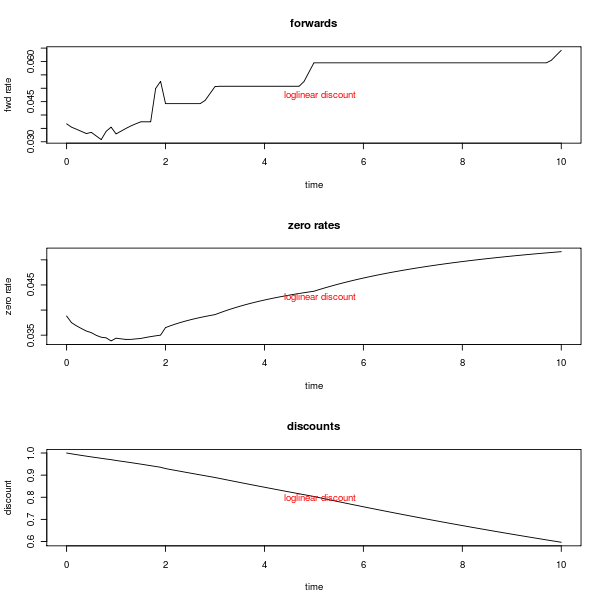
\includegraphics{figures/discountCurve.png}}
\end{center}
\end{frame}

%\begin{frame}[fragile]
%	\frametitle{Fixed Income in RQuantLib}
%	\framesubtitle{Examples: Curve fitting}
%	\begin{itemize}
%		\item DiscountCurve example:		
%
%			\lstset{language=R,basicstyle=\tiny}
%				\begin{lstlisting}		
%params <- list(tradeDate=as.Date('2004-09-20'),
%               settleDate=as.Date('2004-09-22'),
%               interpWhat="discount",
%               interpHow="loglinear")
%tsQuotes <- list(d1w = 0.0382,
%                 d1m = 0.0372,
%                 d3m = 0.0363,
%                 d6m = 0.0353,
%                 d9m = 0.0348,
%                 d1y = 0.0345,
%                 fut2=96.7875,
%                 fut3=96.9875,
%                 fut4=96.6875,
%                 fut5=96.4875,
%                 fut7=96.2875,
%                 s2y = 0.037125,
%                 s3y = 0.0398,
%                 s5y = 0.0443,
%                 s10y = 0.05165,
%                 s15y = 0.055175)
%curves <- DiscountCurve(params, tsQuotes)		
%\end{lstlisting}
%\end{itemize}
%\end{frame}

\begin{frame}
	\frametitle{Fixed Income in RQuantLib}
	\framesubtitle{Examples: Curve fitting with FittedBondCurve function}
Fitting a curve to a set of bonds. The data is taken from codes shipped with QuantLib 0.9.7.
\vskip5pt
\pagecolor{bgcolor}
\noindent
\ttfamily
\hlstd{lengths\ }\hlsym{$<${-}\ }\hlstd{}\hlkwc{c}\hlstd{}\hlsym{(}\hlstd{}\hlnum{2}\hlstd{}\hlsym{,}\hlstd{}\hlnum{4}\hlstd{}\hlsym{,}\hlstd{}\hlnum{6}\hlstd{}\hlsym{,}\hlstd{}\hlnum{8}\hlstd{}\hlsym{,}\hlstd{}\hlnum{10}\hlstd{}\hlsym{,}\hlstd{}\hlnum{12}\hlstd{}\hlsym{,}\hlstd{}\hlnum{14}\hlstd{}\hlsym{,}\hlstd{}\hlnum{16}\hlstd{}\hlsym{,}\hlstd{}\hlnum{18}\hlstd{}\hlsym{,}\hspace*{\fill}\\
\hlstd{}\hlstd{\ \ \ \ \ \ \ \ \ \ \ \ \ }\hlstd{}\hlnum{20}\hlstd{}\hlsym{,}\hlstd{}\hlnum{22}\hlstd{}\hlsym{,}\hlstd{}\hlnum{24}\hlstd{}\hlsym{,}\hlstd{}\hlnum{26}\hlstd{}\hlsym{,}\hlstd{}\hlnum{28}\hlstd{}\hlsym{,}\hlstd{}\hlnum{30}\hlstd{}\hlsym{)}\hspace*{\fill}\\
\hlstd{coupons\ }\hlsym{$<${-}\ }\hlstd{}\hlkwc{c}\hlstd{}\hlsym{(}\hlstd{}\hlnum{0.0200}\hlstd{}\hlsym{,\ }\hlstd{}\hlnum{0.0225}\hlstd{}\hlsym{,\ }\hlstd{}\hlnum{0.0250}\hlstd{}\hlsym{,\ }\hlstd{}\hlnum{0.0275}\hlstd{}\hlsym{,}\hspace*{\fill}\\
\hlstd{}\hlstd{\ \ \ \ \ \ \ \ \ \ \ \ \ }\hlstd{}\hlnum{0.0300}\hlstd{}\hlsym{,\ }\hlstd{}\hlnum{0.0325}\hlstd{}\hlsym{,\ }\hlstd{}\hlnum{0.0350}\hlstd{}\hlsym{,\ }\hlstd{}\hlnum{0.0375}\hlstd{}\hlsym{,}\hspace*{\fill}\\
\hlstd{}\hlstd{\ \ \ \ \ \ \ \ \ \ \ \ \ }\hlstd{}\hlnum{0.0400}\hlstd{}\hlsym{,\ }\hlstd{}\hlnum{0.0425}\hlstd{}\hlsym{,\ }\hlstd{}\hlnum{0.0450}\hlstd{}\hlsym{,\ }\hlstd{}\hlnum{0.0475}\hlstd{}\hlsym{,}\hspace*{\fill}\\
\hlstd{}\hlstd{\ \ \ \ \ \ \ \ \ \ \ \ \ }\hlstd{}\hlnum{0.0500}\hlstd{}\hlsym{,\ }\hlstd{}\hlnum{0.0525}\hlstd{}\hlsym{,\ }\hlstd{}\hlnum{0.0550\ }\hlstd{}\hlsym{)}\hspace*{\fill}\\
\hlstd{marketQuotes\ }\hlsym{$<${-}\ }\hlstd{}\hlkwc{rep}\hlstd{}\hlsym{(}\hlstd{}\hlnum{100}\hlstd{}\hlsym{,\ }\hlstd{}\hlkwc{length}\hlstd{}\hlsym{(}\hlstd{lengths}\hlsym{))}\hspace*{\fill}\\
\hlstd{dateparams\ }\hlsym{$<${-}\ }\hlstd{}\hlkwc{list}\hlstd{}\hlsym{(}\hlstd{settlementDays}\hlsym{=}\hlstd{}\hlnum{0}\hlstd{}\hlsym{,}\hspace*{\fill}\\
\hlstd{}\hlstd{\ \ \ \ \ \ \ \ \ \ \ \ \ \ \ \ \ \ \ }\hlstd{period}\hlsym{=}\hlstd{}\hlstr{"Annual"}\hlstd{}\hlsym{,}\hspace*{\fill}\\
\hlstd{}\hlstd{\ \ \ \ \ \ \ \ \ \ \ \ \ \ \ \ \ \ \ }\hlstd{dayCounter}\hlsym{=}\hlstd{}\hlstr{"ActualActual"}\hlstd{}\hlsym{,}\hspace*{\fill}\\
\hlstd{}\hlstd{\ \ \ \ \ \ \ \ \ \ \ \ \ \ \ \ \ \ \ }\hlstd{businessDayConvention}\hlsym{=}\hlstd{}\hlstr{"Unadjusted"}\hlstd{}\hlsym{)}\hspace*{\fill}\\
\hlstd{curveparams\ }\hlsym{$<${-}\ }\hlstd{}\hlkwc{list}\hlstd{}\hlsym{(}\hlstd{method}\hlsym{=}\hlstd{}\hlstr{"ExponentialSplinesFitting"}\hlstd{}\hlsym{,}\hspace*{\fill}\\
\hlstd{}\hlstd{\ \ \ \ \ \ \ \ \ \ \ \ \ \ \ \ \ \ \ \ }\hlstd{origDate\ }\hlsym{=\ }\hlstd{}\hlkwc{Sys.Date}\hlstd{}\hlsym{())}\hspace*{\fill}\\
\hlstd{}\hlkwc{curve\ }\hlstd{}\hlsym{$<${-}\ }\hlstd{FittedBondCurve}\hlsym{(}\hlstd{curveparams}\hlsym{,\ }\hlstd{lengths}\hlsym{,}\hspace*{\fill}\\
\hlstd{}\hlstd{\ \ \ \ \ \ \ \ \ \ \ \ \ \ \ \ \ \ \ \ \ \ \ \ \ }\hlstd{coupons}\hlsym{,\ }\hlstd{marketQuotes}\hlsym{,}\hspace*{\fill}\\
\hlstd{}\hlstd{\ \ \ \ \ \ \ \ \ \ \ \ \ \ \ \ \ \ \ \ \ \ \ \ \ }\hlstd{dateparams}\hlsym{)}\hspace*{\fill}\\
\mbox{}
\normalfont
\end{frame}

\begin{frame}
	\frametitle{Fixed Income in RQuantLib}
	\framesubtitle{Examples: Curve fitting with FittedBondCurve function}
\pagecolor{bgcolor}
\noindent
\scriptsize
\ttfamily
\vskip5pt
\hlstd{}\hlkwc{library}\hlstd{}\hlsym{(}\hlstd{zoo}\hlsym{)}\hspace*{\fill}\\
\hlstd{z\ }\hlsym{$<${-}\ }\hlstd{zoo}\hlsym{(}\hlstd{}\hlkwc{curve}\hlstd{\$}\hlkwc{table}\hlstd{\$zeroRates}\hlsym{,\ }\hlstd{order.by}\hlsym{=}\hlstd{}\hlkwc{curve}\hlstd{\$}\hlkwc{table}\hlstd{\$}\hlkwc{date}\hlstd{}\hlsym{)}\hspace*{\fill}\\
\hlstd{}\hlkwc{plot}\hlstd{}\hlsym{(}\hlstd{z, xlab='Date', ylab='Zero Rates')}
\normalfont
\begin{center}
\resizebox{75mm}{!}{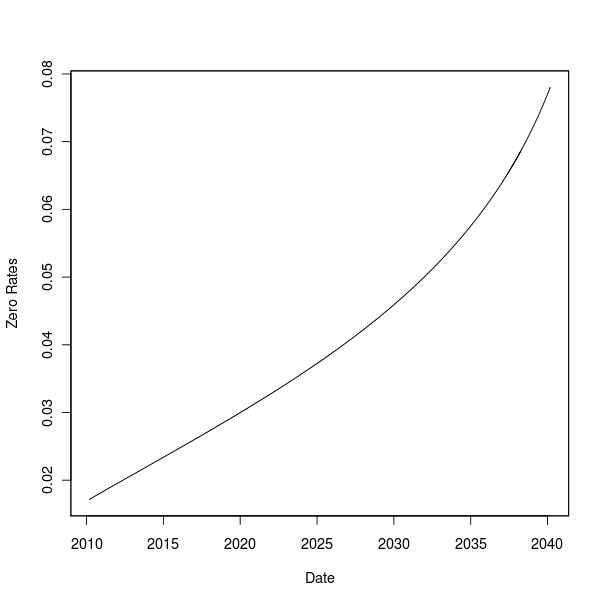
\includegraphics{figures/fittedBondCurve.png}}
\end{center}
\end{frame}


%\begin{frame}[fragile]
%	\frametitle{Fixed Income in RQuantLib}
%	\framesubtitle{Examples: Curve fitting}
%	\begin{itemize}
%		\item FittedBondCurve example:
%			\lstset{language=R,basicstyle=\tiny}
%				\begin{lstlisting}
%lengths <- c(2,4,6,8,10,12,14,16,18,20,22,24,26,28,30)
%coupons <- c(0.0200, 0.0225, 0.0250, 0.0275, 0.0300,
%         	 0.0325, 0.0350, 0.0375, 0.0400, 0.0425,
%             0.0450, 0.0475, 0.0500, 0.0525, 0.0550 )
%marketQuotes <- rep(100, length(lengths))
%dateparams <- list(settlementDays=0, period="Annual", 
%                             dayCounter="ActualActual", 
%                             businessDayConvention ="Unadjusted")
%curveparams <- list(method="ExponentialSplinesFitting", 
%                                origDate = Sys.Date())
%curve <- FittedBondCurve(curveparams, lengths, coupons, marketQuotes, dateparams)
%library(zoo)
%z <- zoo(curve$table$zeroRates, order.by=curve$table$date)
%plot(z)
%				\end{lstlisting}		
%
%\end{itemize}
%\end{frame}
\begin{frame}
	\frametitle{Fixed Income in RQuantLib}
	\framesubtitle{Examples: Bond pricing}	
In this example, we construct a bond discounting term structure and a swap term structure then use them to price a zero coupon bond and a fixed rate bond. First, we will walk quickly through the QuantLib's implementation.
\vskip5pt
\pagecolor{bgcolor}
\tiny
\noindent
\ttfamily
\hlstd{}\hlslc{//\ the\ only\ header\ you\ need\ to\ use\ QuantLib}\hspace*{\fill}\\
\hlstd{}\hldir{\#include\ $<$ql/quantlib.hpp$>$}\hspace*{\fill}\\
\hlstd{}\hspace*{\fill}\\
\hldir{\#include\ $<$boost/timer.hpp$>$}\hspace*{\fill}\\
\hlstd{}\hldir{\#include\ $<$iostream$>$}\hspace*{\fill}\\
\hlstd{}\hldir{\#include\ $<$iomanip$>$}\hspace*{\fill}\\
\hlstd{}\hspace*{\fill}\\
\hlkwa{using\ namespace\ }\hlstd{QuantLib}\hlsym{;}\hspace*{\fill}\\
\hlstd{}\hspace*{\fill}\\
\hldir{\#if\ defined(QL\textunderscore ENABLE\textunderscore SESSIONS)}\hspace*{\fill}\\
\hlstd{}\hlkwa{namespace\ }\hlstd{QuantLib\ }\hlsym{\{}\hspace*{\fill}\\
\hlstd{\hspace*{\fill}\\
Integer\ }\hlkwd{sessionId}\hlstd{}\hlsym{()\ \{\ }\hlstd{}\hlkwa{return\ }\hlstd{}\hlnum{0}\hlstd{}\hlsym{;\ \}}\hspace*{\fill}\\
\hlstd{}\hspace*{\fill}\\
\hlsym{\}}\hspace*{\fill}\\
\hlstd{}\hldir{\#endif}\hspace*{\fill}\\
\hlstd{}\hspace*{\fill}\\
\hspace*{\fill}\\
\hlkwb{int\ }\hlstd{}\hlkwd{main}\hlstd{}\hlsym{(}\hlstd{}\hlkwb{int}\hlstd{}\hlsym{,\ }\hlstd{}\hlkwb{char}\hlstd{}\hlsym{{*}\ {[}{]})\ \{}\hspace*{\fill}\\
\hlstd{\hspace*{\fill}\\
}\hlstd{\ \ \ \ }\hlstd{}\hlkwa{try\ }\hlstd{}\hlsym{\{}\hspace*{\fill}\\
\hlstd{\hspace*{\fill}\\
}\hlstd{\ \ \ \ \ \ \ \ }\hlstd{boost}\hlsym{::}\hlstd{timer\ timer}\hlsym{;}\hspace*{\fill}\\
\hlstd{}\hlstd{\ \ \ \ \ \ \ \ }\hlstd{std}\hlsym{::}\hlstd{cout\ }\hlsym{$<$$<$\ }\hlstd{std}\hlsym{::}\hlstd{endl}\hlsym{;}\hspace*{\fill}\\
\hlstd{\hspace*{\fill}\\
}\hlstd{\ \ \ \ \ \ \ \ }\hlstd{}\hlcom{/{*}{*}{*}{*}{*}{*}{*}{*}{*}{*}{*}{*}{*}{*}{*}{*}{*}{*}{*}{*}{*}}\hspace*{\fill}\\
\hlcom{}\hlstd{\ \ \ \ \ \ \ \ \ }\hlcom{{*}{*}{*}}\hlstd{\ \ }\hlcom{MARKET\ DATA}\hlstd{\ \ }\hlcom{{*}{*}{*}}\hspace*{\fill}\\
\hlcom{}\hlstd{\ \ \ \ \ \ \ \ \ }\hlcom{{*}{*}{*}{*}{*}{*}{*}{*}{*}{*}{*}{*}{*}{*}{*}{*}{*}{*}{*}{*}{*}/}\hlstd{\hspace*{\fill}\\
\hspace*{\fill}\\
}\hlstd{\ \ \ \ \ \ \ \ }\hlstd{Calendar\ calendar\ }\hlsym{=\ }\hlstd{}\hlkwd{TARGET}\hlstd{}\hlsym{();}\hspace*{\fill}\\
\hlstd{\hspace*{\fill}\\
}\hlstd{\ \ \ \ \ \ \ \ }\hlstd{Date\ }\hlkwd{settlementDate}\hlstd{}\hlsym{(}\hlstd{}\hlnum{18}\hlstd{}\hlsym{,\ }\hlstd{September}\hlsym{,\ }\hlstd{}\hlnum{2008}\hlstd{}\hlsym{);}\hspace*{\fill}\\
\hlstd{}\hlstd{\ \ \ \ \ \ \ \ }\hlstd{}\hlslc{//\ must\ be\ a\ business\ day}\hspace*{\fill}\\
\hlstd{}\hlstd{\ \ \ \ \ \ \ \ }\hlstd{settlementDate\ }\hlsym{=\ }\hlstd{calendar}\hlsym{.}\hlstd{}\hlkwd{adjust}\hlstd{}\hlsym{(}\hlstd{settlementDate}\hlsym{);}\hspace*{\fill}\\
\hlstd{\hspace*{\fill}\\
}\hlstd{\ \ \ \ \ \ \ \ }\hlstd{Integer\ fixingDays\ }\hlsym{=\ }\hlstd{}\hlnum{3}\hlstd{}\hlsym{;}\hspace*{\fill}\\
\hlstd{}\hlstd{\ \ \ \ \ \ \ \ }\hlstd{Natural\ settlementDays\ }\hlsym{=\ }\hlstd{}\hlnum{3}\hlstd{}\hlsym{;}\hspace*{\fill}\\
\hlstd{\hspace*{\fill}\\
}\hlstd{\ \ \ \ \ \ \ \ }\hlstd{Date\ todaysDate\ }\hlsym{=\ }\hlstd{calendar}\hlsym{.}\hlstd{}\hlkwd{advance}\hlstd{}\hlsym{(}\hlstd{settlementDate}\hlsym{,\ {-}}\hlstd{fixingDays}\hlsym{,\ }\hlstd{Days}\hlsym{);}\hspace*{\fill}\\
\hlstd{}\hlstd{\ \ \ \ \ \ \ \ }\hlstd{}\hlslc{//\ nothing\ to\ do\ with\ Date::todaysDate}\hspace*{\fill}\\
\hlstd{}\hlstd{\ \ \ \ \ \ \ \ }\hlstd{Settings}\hlsym{::}\hlstd{}\hlkwd{instance}\hlstd{}\hlsym{().}\hlstd{}\hlkwd{evaluationDate}\hlstd{}\hlsym{()\ =\ }\hlstd{todaysDate}\hlsym{;}\hspace*{\fill}\\
\hlstd{\hspace*{\fill}\\
}\hlstd{\ \ \ \ \ \ \ \ }\hlstd{std}\hlsym{::}\hlstd{cout\ }\hlsym{$<$$<$\ }\hlstd{}\hlstr{"Today:\ "}\hlstd{\ }\hlsym{$<$$<$\ }\hlstd{todaysDate}\hlsym{.}\hlstd{}\hlkwd{weekday}\hlstd{}\hlsym{()}\hspace*{\fill}\\
\hlstd{}\hlstd{\ \ \ \ \ \ \ \ }\hlstd{}\hlsym{$<$$<$\ }\hlstd{}\hlstr{",\ "}\hlstd{\ }\hlsym{$<$$<$\ }\hlstd{todaysDate\ }\hlsym{$<$$<$\ }\hlstd{std}\hlsym{::}\hlstd{endl}\hlsym{;}\hspace*{\fill}\\
\hlstd{\hspace*{\fill}\\
}\hlstd{\ \ \ \ \ \ \ \ }\hlstd{std}\hlsym{::}\hlstd{cout\ }\hlsym{$<$$<$\ }\hlstd{}\hlstr{"Settlement\ date:\ "}\hlstd{\ }\hlsym{$<$$<$\ }\hlstd{settlementDate}\hlsym{.}\hlstd{}\hlkwd{weekday}\hlstd{}\hlsym{()}\hspace*{\fill}\\
\hlstd{}\hlstd{\ \ \ \ \ \ \ \ }\hlstd{}\hlsym{$<$$<$\ }\hlstd{}\hlstr{",\ "}\hlstd{\ }\hlsym{$<$$<$\ }\hlstd{settlementDate\ }\hlsym{$<$$<$\ }\hlstd{std}\hlsym{::}\hlstd{endl}\hlsym{;}\hspace*{\fill}\\
\hlstd{\hspace*{\fill}\\
\hspace*{\fill}\\
}\hlstd{\ \ \ \ \ \ \ \ }\hlstd{}\hlslc{//\ Building\ of\ the\ bonds\ discounting\ yield\ curve}\hspace*{\fill}\\
\hlstd{\hspace*{\fill}\\
}\hlstd{\ \ \ \ \ \ \ \ }\hlstd{}\hlcom{/{*}{*}{*}{*}{*}{*}{*}{*}{*}{*}{*}{*}{*}{*}{*}{*}{*}{*}{*}{*}{*}}\hspace*{\fill}\\
\hlcom{}\hlstd{\ \ \ \ \ \ \ \ \ }\hlcom{{*}{*}{*}}\hlstd{\ \ }\hlcom{RATE\ HELPERS\ {*}{*}{*}}\hspace*{\fill}\\
\hlcom{}\hlstd{\ \ \ \ \ \ \ \ \ }\hlcom{{*}{*}{*}{*}{*}{*}{*}{*}{*}{*}{*}{*}{*}{*}{*}{*}{*}{*}{*}{*}{*}/}\hlstd{\hspace*{\fill}\\
\hspace*{\fill}\\
}\hlstd{\ \ \ \ \ \ \ \ }\hlstd{}\hlslc{//\ RateHelpers\ are\ built\ from\ the\ above\ quotes\ together\ with}\hspace*{\fill}\\
\hlstd{}\hlstd{\ \ \ \ \ \ \ \ }\hlstd{}\hlslc{//\ other\ instrument\ dependant\ infos.}\hlstd{\ \ }\hlslc{Quotes\ are\ passed\ in}\hspace*{\fill}\\
\hlstd{}\hlstd{\ \ \ \ \ \ \ \ }\hlstd{}\hlslc{//\ relinkable\ handles\ which\ could\ be\ relinked\ to\ some\ other}\hspace*{\fill}\\
\hlstd{}\hlstd{\ \ \ \ \ \ \ \ }\hlstd{}\hlslc{//\ data\ source\ later.}\hspace*{\fill}\\
\hlstd{\hspace*{\fill}\\
}\hlstd{\ \ \ \ \ \ \ \ }\hlstd{}\hlslc{//\ Common\ data}\hspace*{\fill}\\
\hlstd{\hspace*{\fill}\\
\hspace*{\fill}\\
}\hlstd{\ \ \ \ \ \ \ \ \ }\hlstd{DayCounter\ zcBondsDayCounter\ }\hlsym{=\ }\hlstd{}\hlkwd{Actual365Fixed}\hlstd{}\hlsym{();}\hspace*{\fill}\\
\hlstd{\hspace*{\fill}\\
}\hlstd{\ \ \ \ \ \ \ \ \ }\hlstd{boost}\hlsym{::}\hlstd{shared\textunderscore ptr}\hlsym{$<$}\hlstd{RateHelper}\hlsym{$>$\ }\hlstd{}\hlkwd{zc3m}\hlstd{}\hlsym{(}\hlstd{}\hlkwa{new\ }\hlstd{}\hlkwd{DepositRateHelper}\hlstd{}\hlsym{(}\hspace*{\fill}\\
\hlstd{}\hlstd{\ \ \ \ \ \ \ \ \ \ \ \ \ \ \ \ \ }\hlstd{Handle}\hlsym{$<$}\hlstd{Quote}\hlsym{$>$(}\hlstd{zc3mRate}\hlsym{),}\hspace*{\fill}\\
\hlstd{}\hlstd{\ \ \ \ \ \ \ \ \ \ \ \ \ \ \ \ \ }\hlstd{}\hlnum{3}\hlstd{}\hlsym{{*}}\hlstd{Months}\hlsym{,\ }\hlstd{fixingDays}\hlsym{,}\hspace*{\fill}\\
\hlstd{}\hlstd{\ \ \ \ \ \ \ \ \ \ \ \ \ \ \ \ \ }\hlstd{calendar}\hlsym{,\ }\hlstd{ModifiedFollowing}\hlsym{,}\hspace*{\fill}\\
\hlstd{}\hlstd{\ \ \ \ \ \ \ \ \ \ \ \ \ \ \ \ \ }\hlstd{}\hlkwa{true}\hlstd{}\hlsym{,\ }\hlstd{zcBondsDayCounter}\hlsym{));}\hspace*{\fill}\\
\hlstd{}\hlstd{\ \ \ \ \ \ \ \ \ }\hlstd{boost}\hlsym{::}\hlstd{shared\textunderscore ptr}\hlsym{$<$}\hlstd{RateHelper}\hlsym{$>$\ }\hlstd{}\hlkwd{zc6m}\hlstd{}\hlsym{(}\hlstd{}\hlkwa{new\ }\hlstd{}\hlkwd{DepositRateHelper}\hlstd{}\hlsym{(}\hspace*{\fill}\\
\hlstd{}\hlstd{\ \ \ \ \ \ \ \ \ \ \ \ \ \ \ \ \ }\hlstd{Handle}\hlsym{$<$}\hlstd{Quote}\hlsym{$>$(}\hlstd{zc6mRate}\hlsym{),}\hspace*{\fill}\\
\hlstd{}\hlstd{\ \ \ \ \ \ \ \ \ \ \ \ \ \ \ \ \ }\hlstd{}\hlnum{6}\hlstd{}\hlsym{{*}}\hlstd{Months}\hlsym{,\ }\hlstd{fixingDays}\hlsym{,}\hspace*{\fill}\\
\hlstd{}\hlstd{\ \ \ \ \ \ \ \ \ \ \ \ \ \ \ \ \ }\hlstd{calendar}\hlsym{,\ }\hlstd{ModifiedFollowing}\hlsym{,}\hspace*{\fill}\\
\hlstd{}\hlstd{\ \ \ \ \ \ \ \ \ \ \ \ \ \ \ \ \ }\hlstd{}\hlkwa{true}\hlstd{}\hlsym{,\ }\hlstd{zcBondsDayCounter}\hlsym{));}\hspace*{\fill}\\
\hlstd{}\hlstd{\ \ \ \ \ \ \ \ \ }\hlstd{boost}\hlsym{::}\hlstd{shared\textunderscore ptr}\hlsym{$<$}\hlstd{RateHelper}\hlsym{$>$\ }\hlstd{}\hlkwd{zc1y}\hlstd{}\hlsym{(}\hlstd{}\hlkwa{new\ }\hlstd{}\hlkwd{DepositRateHelper}\hlstd{}\hlsym{(}\hspace*{\fill}\\
\hlstd{}\hlstd{\ \ \ \ \ \ \ \ \ \ \ \ \ \ \ \ \ }\hlstd{Handle}\hlsym{$<$}\hlstd{Quote}\hlsym{$>$(}\hlstd{zc1yRate}\hlsym{),}\hspace*{\fill}\\
\hlstd{}\hlstd{\ \ \ \ \ \ \ \ \ \ \ \ \ \ \ \ \ }\hlstd{}\hlnum{1}\hlstd{}\hlsym{{*}}\hlstd{Years}\hlsym{,\ }\hlstd{fixingDays}\hlsym{,}\hspace*{\fill}\\
\hlstd{}\hlstd{\ \ \ \ \ \ \ \ \ \ \ \ \ \ \ \ \ }\hlstd{calendar}\hlsym{,\ }\hlstd{ModifiedFollowing}\hlsym{,}\hspace*{\fill}\\
\hlstd{}\hlstd{\ \ \ \ \ \ \ \ \ \ \ \ \ \ \ \ \ }\hlstd{}\hlkwa{true}\hlstd{}\hlsym{,\ }\hlstd{zcBondsDayCounter}\hlsym{));}\hspace*{\fill}\\
\hlstd{\hspace*{\fill}\\
}\hlstd{\ \ \ \ \ \ \ \ }\hlstd{}\hlslc{//\ setup\ bonds}\hspace*{\fill}\\
\hlstd{}\hlstd{\ \ \ \ \ \ \ \ }\hlstd{Real\ redemption\ }\hlsym{=\ }\hlstd{}\hlnum{100.0}\hlstd{}\hlsym{;}\hspace*{\fill}\\
\hlstd{\hspace*{\fill}\\
}\hlstd{\ \ \ \ \ \ \ \ }\hlstd{}\hlkwb{const\ }\hlstd{Size\ numberOfBonds\ }\hlsym{=\ }\hlstd{}\hlnum{5}\hlstd{}\hlsym{;}\hspace*{\fill}\\
\hlstd{\hspace*{\fill}\\
}\hlstd{\ \ \ \ \ \ \ \ }\hlstd{Date\ issueDates}\hlsym{{[}{]}\ =\ \{}\hspace*{\fill}\\
\hlstd{}\hlstd{\ \ \ \ \ \ \ \ \ \ \ \ \ \ \ \ }\hlstd{todaysDate\ }\hlsym{+\ }\hlstd{}\hlnum{3}\hlstd{}\hlsym{,}\hspace*{\fill}\\
\hlstd{}\hlstd{\ \ \ \ \ \ \ \ \ \ \ \ \ \ \ \ }\hlstd{todaysDate\ }\hlsym{+\ }\hlstd{}\hlnum{3}\hlstd{}\hlsym{,}\hspace*{\fill}\\
\hlstd{}\hlstd{\ \ \ \ \ \ \ \ \ \ \ \ \ \ \ \ }\hlstd{todaysDate\ }\hlsym{+\ }\hlstd{}\hlnum{3}\hlstd{}\hlsym{,}\hspace*{\fill}\\
\hlstd{}\hlstd{\ \ \ \ \ \ \ \ \ \ \ \ \ \ \ \ }\hlstd{todaysDate\ }\hlsym{+\ }\hlstd{}\hlnum{3}\hlstd{}\hlsym{,}\hspace*{\fill}\\
\hlstd{}\hlstd{\ \ \ \ \ \ \ \ \ \ \ \ \ \ \ \ }\hlstd{todaysDate\ }\hlsym{+\ }\hlstd{}\hlnum{3}\hspace*{\fill}\\
\hlstd{}\hlstd{\ \ \ \ \ \ \ \ }\hlstd{}\hlsym{\};}\hspace*{\fill}\\
\hlstd{\hspace*{\fill}\\
}\hlstd{\ \ \ \ \ \ \ \ }\hlstd{Date\ maturities}\hlsym{{[}{]}\ =\ \{}\hspace*{\fill}\\
\hlstd{}\hlstd{\ \ \ \ \ \ \ \ \ \ \ \ \ \ \ \ }\hlstd{calendar}\hlsym{.}\hlstd{}\hlkwd{advance}\hlstd{}\hlsym{(}\hlstd{todaysDate\ }\hlsym{+\ }\hlstd{}\hlnum{3}\hlstd{}\hlsym{,\ }\hlstd{}\hlnum{5}\hlstd{}\hlsym{,\ }\hlstd{Years}\hlsym{),}\hspace*{\fill}\\
\hlstd{}\hlstd{\ \ \ \ \ \ \ \ \ \ \ \ \ \ \ \ }\hlstd{calendar}\hlsym{.}\hlstd{}\hlkwd{advance}\hlstd{}\hlsym{(}\hlstd{todaysDate\ }\hlsym{+\ }\hlstd{}\hlnum{3}\hlstd{}\hlsym{,\ }\hlstd{}\hlnum{6}\hlstd{}\hlsym{,\ }\hlstd{Years}\hlsym{),}\hspace*{\fill}\\
\hlstd{}\hlstd{\ \ \ \ \ \ \ \ \ \ \ \ \ \ \ \ }\hlstd{calendar}\hlsym{.}\hlstd{}\hlkwd{advance}\hlstd{}\hlsym{(}\hlstd{todaysDate\ }\hlsym{+\ }\hlstd{}\hlnum{3}\hlstd{}\hlsym{,\ }\hlstd{}\hlnum{7}\hlstd{}\hlsym{,\ }\hlstd{Years}\hlsym{),}\hspace*{\fill}\\
\hlstd{}\hlstd{\ \ \ \ \ \ \ \ \ \ \ \ \ \ \ \ }\hlstd{calendar}\hlsym{.}\hlstd{}\hlkwd{advance}\hlstd{}\hlsym{(}\hlstd{todaysDate\ }\hlsym{+\ }\hlstd{}\hlnum{3}\hlstd{}\hlsym{,\ }\hlstd{}\hlnum{16}\hlstd{}\hlsym{,\ }\hlstd{Years}\hlsym{),}\hspace*{\fill}\\
\hlstd{}\hlstd{\ \ \ \ \ \ \ \ \ \ \ \ \ \ \ \ }\hlstd{calendar}\hlsym{.}\hlstd{}\hlkwd{advance}\hlstd{}\hlsym{(}\hlstd{todaysDate\ }\hlsym{+\ }\hlstd{}\hlnum{3}\hlstd{}\hlsym{,\ }\hlstd{}\hlnum{48}\hlstd{}\hlsym{,\ }\hlstd{Years}\hlsym{)}\hspace*{\fill}\\
\hlstd{}\hlstd{\ \ \ \ \ \ \ \ }\hlstd{}\hlsym{\};}\hspace*{\fill}\\
\hlstd{\hspace*{\fill}\\
}\hlstd{\ \ \ \ \ \ \ \ }\hlstd{Real\ couponRates}\hlsym{{[}{]}\ =\ \{}\hspace*{\fill}\\
\hlstd{}\hlstd{\ \ \ \ \ \ \ \ \ \ \ \ \ \ \ \ }\hlstd{}\hlnum{0.02375}\hlstd{}\hlsym{,}\hspace*{\fill}\\
\hlstd{}\hlstd{\ \ \ \ \ \ \ \ \ \ \ \ \ \ \ \ }\hlstd{}\hlnum{0.04625}\hlstd{}\hlsym{,}\hspace*{\fill}\\
\hlstd{}\hlstd{\ \ \ \ \ \ \ \ \ \ \ \ \ \ \ \ }\hlstd{}\hlnum{0.03125}\hlstd{}\hlsym{,}\hspace*{\fill}\\
\hlstd{}\hlstd{\ \ \ \ \ \ \ \ \ \ \ \ \ \ \ \ }\hlstd{}\hlnum{0.04000}\hlstd{}\hlsym{,}\hspace*{\fill}\\
\hlstd{}\hlstd{\ \ \ \ \ \ \ \ \ \ \ \ \ \ \ \ }\hlstd{}\hlnum{0.04500}\hspace*{\fill}\\
\hlstd{}\hlstd{\ \ \ \ \ \ \ \ }\hlstd{}\hlsym{\};}\hspace*{\fill}\\
\hlstd{\hspace*{\fill}\\
}\hlstd{\ \ \ \ \ \ \ \ }\hlstd{Real\ marketQuotes}\hlsym{{[}{]}\ =\ \{}\hspace*{\fill}\\
\hlstd{}\hlstd{\ \ \ \ \ \ \ \ \ \ \ \ \ \ \ \ }\hlstd{}\hlnum{100.390625}\hlstd{}\hlsym{,}\hspace*{\fill}\\
\hlstd{}\hlstd{\ \ \ \ \ \ \ \ \ \ \ \ \ \ \ \ }\hlstd{}\hlnum{106.21875}\hlstd{}\hlsym{,}\hspace*{\fill}\\
\hlstd{}\hlstd{\ \ \ \ \ \ \ \ \ \ \ \ \ \ \ \ }\hlstd{}\hlnum{100.59375}\hlstd{}\hlsym{,}\hspace*{\fill}\\
\hlstd{}\hlstd{\ \ \ \ \ \ \ \ \ \ \ \ \ \ \ \ }\hlstd{}\hlnum{101.6875}\hlstd{}\hlsym{,}\hspace*{\fill}\\
\hlstd{}\hlstd{\ \ \ \ \ \ \ \ \ \ \ \ \ \ \ \ }\hlstd{}\hlnum{102.140625}\hspace*{\fill}\\
\hlstd{}\hlstd{\ \ \ \ \ \ \ \ }\hlstd{}\hlsym{\};}\hspace*{\fill}\\
\hlstd{\hspace*{\fill}\\
}\hlstd{\ \ \ \ \ \ \ \ }\hlstd{std}\hlsym{::}\hlstd{vector}\hlsym{$<$\ }\hlstd{boost}\hlsym{::}\hlstd{shared\textunderscore ptr}\hlsym{$<$}\hlstd{SimpleQuote}\hlsym{$>$\ $>$\ }\hlstd{quote}\hlsym{;}\hspace*{\fill}\\
\hlstd{}\hlstd{\ \ \ \ \ \ \ \ }\hlstd{}\hlkwa{for\ }\hlstd{}\hlsym{(}\hlstd{Size\ i}\hlsym{=}\hlstd{}\hlnum{0}\hlstd{}\hlsym{;\ }\hlstd{i}\hlsym{$<$}\hlstd{numberOfBonds}\hlsym{;\ }\hlstd{i}\hlsym{++)\ \{}\hspace*{\fill}\\
\hlstd{}\hlstd{\ \ \ \ \ \ \ \ \ \ \ \ }\hlstd{boost}\hlsym{::}\hlstd{shared\textunderscore ptr}\hlsym{$<$}\hlstd{SimpleQuote}\hlsym{$>$\ }\hlstd{}\hlkwd{cp}\hlstd{}\hlsym{(}\hlstd{}\hlkwa{new\ }\hlstd{}\hlkwd{SimpleQuote}\hlstd{}\hlsym{(}\hlstd{marketQuotes}\hlsym{{[}}\hlstd{i}\hlsym{{]}));}\hspace*{\fill}\\
\hlstd{}\hlstd{\ \ \ \ \ \ \ \ \ \ \ \ }\hlstd{quote}\hlsym{.}\hlstd{}\hlkwd{push\textunderscore back}\hlstd{}\hlsym{(}\hlstd{cp}\hlsym{);}\hspace*{\fill}\\
\hlstd{}\hlstd{\ \ \ \ \ \ \ \ }\hlstd{}\hlsym{\}}\hspace*{\fill}\\
\hlstd{\hspace*{\fill}\\
}\hlstd{\ \ \ \ \ \ \ \ }\hlstd{RelinkableHandle}\hlsym{$<$}\hlstd{Quote}\hlsym{$>$\ }\hlstd{quoteHandle}\hlsym{{[}}\hlstd{numberOfBonds}\hlsym{{]};}\hspace*{\fill}\\
\hlstd{}\hlstd{\ \ \ \ \ \ \ \ }\hlstd{}\hlkwa{for\ }\hlstd{}\hlsym{(}\hlstd{Size\ i}\hlsym{=}\hlstd{}\hlnum{0}\hlstd{}\hlsym{;\ }\hlstd{i}\hlsym{$<$}\hlstd{numberOfBonds}\hlsym{;\ }\hlstd{i}\hlsym{++)\ \{}\hspace*{\fill}\\
\hlstd{}\hlstd{\ \ \ \ \ \ \ \ \ \ \ \ }\hlstd{quoteHandle}\hlsym{{[}}\hlstd{i}\hlsym{{]}.}\hlstd{}\hlkwd{linkTo}\hlstd{}\hlsym{(}\hlstd{quote}\hlsym{{[}}\hlstd{i}\hlsym{{]});}\hspace*{\fill}\\
\hlstd{}\hlstd{\ \ \ \ \ \ \ \ }\hlstd{}\hlsym{\}}\hspace*{\fill}\\
\hlstd{\hspace*{\fill}\\
}\hlstd{\ \ \ \ \ \ \ \ }\hlstd{}\hlslc{//\ Definition\ of\ the\ rate\ helpers}\hspace*{\fill}\\
\hlstd{}\hlstd{\ \ \ \ \ \ \ \ }\hlstd{std}\hlsym{::}\hlstd{vector}\hlsym{$<$}\hlstd{boost}\hlsym{::}\hlstd{shared\textunderscore ptr}\hlsym{$<$}\hlstd{FixedRateBondHelper}\hlsym{$>$\ $>$\ }\hlstd{bondsHelpers}\hlsym{;}\hspace*{\fill}\\
\hlstd{\hspace*{\fill}\\
}\hlstd{\ \ \ \ \ \ \ \ }\hlstd{}\hlkwa{for\ }\hlstd{}\hlsym{(}\hlstd{Size\ i}\hlsym{=}\hlstd{}\hlnum{0}\hlstd{}\hlsym{;\ }\hlstd{i}\hlsym{$<$}\hlstd{numberOfBonds}\hlsym{;\ }\hlstd{i}\hlsym{++)\ \{}\hspace*{\fill}\\
\hlstd{\hspace*{\fill}\\
}\hlstd{\ \ \ \ \ \ \ \ \ \ \ \ }\hlstd{Schedule\ }\hlkwd{schedule}\hlstd{}\hlsym{(}\hlstd{issueDates}\hlsym{{[}}\hlstd{i}\hlsym{{]},\ }\hlstd{maturities}\hlsym{{[}}\hlstd{i}\hlsym{{]},\ }\hlstd{}\hlkwd{Period}\hlstd{}\hlsym{(}\hlstd{Semiannual}\hlsym{),\ }\hlstd{}\hlkwd{UnitedStates}\hlstd{}\hlsym{(}\hlstd{UnitedStates}\hlsym{::}\hlstd{GovernmentBond}\hlsym{),}\hspace*{\fill}\\
\hlstd{}\hlstd{\ \ \ \ \ \ \ \ \ \ \ \ \ \ \ \ \ \ \ \ }\hlstd{Unadjusted}\hlsym{,\ }\hlstd{Unadjusted}\hlsym{,\ }\hlstd{DateGeneration}\hlsym{::}\hlstd{Backward}\hlsym{,\ }\hlstd{}\hlkwa{false}\hlstd{}\hlsym{);}\hspace*{\fill}\\
\hlstd{\hspace*{\fill}\\
}\hlstd{\ \ \ \ \ \ \ \ \ \ \ \ }\hlstd{boost}\hlsym{::}\hlstd{shared\textunderscore ptr}\hlsym{$<$}\hlstd{FixedRateBondHelper}\hlsym{$>$\ }\hlstd{}\hlkwd{bondHelper}\hlstd{}\hlsym{(}\hlstd{}\hlkwa{new\ }\hlstd{}\hlkwd{FixedRateBondHelper}\hlstd{}\hlsym{(}\hspace*{\fill}\\
\hlstd{}\hlstd{\ \ \ \ \ \ \ \ \ \ \ \ \ \ \ \ \ \ \ \ }\hlstd{quoteHandle}\hlsym{{[}}\hlstd{i}\hlsym{{]},}\hspace*{\fill}\\
\hlstd{}\hlstd{\ \ \ \ \ \ \ \ \ \ \ \ \ \ \ \ \ \ \ \ }\hlstd{settlementDays}\hlsym{,}\hspace*{\fill}\\
\hlstd{}\hlstd{\ \ \ \ \ \ \ \ \ \ \ \ \ \ \ \ \ \ \ \ }\hlstd{}\hlnum{100.0}\hlstd{}\hlsym{,}\hspace*{\fill}\\
\hlstd{}\hlstd{\ \ \ \ \ \ \ \ \ \ \ \ \ \ \ \ \ \ \ \ }\hlstd{schedule}\hlsym{,}\hspace*{\fill}\\
\hlstd{}\hlstd{\ \ \ \ \ \ \ \ \ \ \ \ \ \ \ \ \ \ \ \ }\hlstd{std}\hlsym{::}\hlstd{vector}\hlsym{$<$}\hlstd{Rate}\hlsym{$>$(}\hlstd{}\hlnum{1}\hlstd{}\hlsym{,}\hlstd{couponRates}\hlsym{{[}}\hlstd{i}\hlsym{{]}),}\hspace*{\fill}\\
\hlstd{}\hlstd{\ \ \ \ \ \ \ \ \ \ \ \ \ \ \ \ \ \ \ \ }\hlstd{}\hlkwd{ActualActual}\hlstd{}\hlsym{(}\hlstd{ActualActual}\hlsym{::}\hlstd{Bond}\hlsym{),}\hspace*{\fill}\\
\hlstd{}\hlstd{\ \ \ \ \ \ \ \ \ \ \ \ \ \ \ \ \ \ \ \ }\hlstd{Unadjusted}\hlsym{,}\hspace*{\fill}\\
\hlstd{}\hlstd{\ \ \ \ \ \ \ \ \ \ \ \ \ \ \ \ \ \ \ \ }\hlstd{redemption}\hlsym{,}\hspace*{\fill}\\
\hlstd{}\hlstd{\ \ \ \ \ \ \ \ \ \ \ \ \ \ \ \ \ \ \ \ }\hlstd{issueDates}\hlsym{{[}}\hlstd{i}\hlsym{{]}));}\hspace*{\fill}\\
\hlstd{\hspace*{\fill}\\
}
\hlstd{\ \ \ \ \ \ \ \ \ \ \ \ }\hlstd{bondsHelpers}\hlsym{.}\hlstd{}\hlkwd{push\textunderscore back}\hlstd{}\hlsym{(}\hlstd{bondHelper}\hlsym{);}\hspace*{\fill}\\
\hlstd{}\hlstd{\ \ \ \ \ \ \ \ }\hlstd{}\hlsym{\}}\hspace*{\fill}\\
\hlstd{\hspace*{\fill}\\
}\hlstd{\ \ \ \ \ \ \ \ }\hlstd{}\hlcom{/{*}{*}{*}{*}{*}{*}{*}{*}{*}{*}{*}{*}{*}{*}{*}{*}{*}{*}{*}{*}{*}}\hspace*{\fill}\\
\hlcom{}\hlstd{\ \ \ \ \ \ \ \ \ }\hlcom{{*}{*}}\hlstd{\ \ }\hlcom{CURVE\ BUILDING\ {*}{*}}\hspace*{\fill}\\
\hlcom{}\hlstd{\ \ \ \ \ \ \ \ \ }\hlcom{{*}{*}{*}{*}{*}{*}{*}{*}{*}{*}{*}{*}{*}{*}{*}{*}{*}{*}{*}{*}{*}/}\hlstd{\hspace*{\fill}\\
\hspace*{\fill}\\
}\hlstd{\ \ \ \ \ \ \ \ \ }\hlstd{}\hlslc{//\ Any\ DayCounter\ would\ be\ fine.}\hspace*{\fill}\\
\hlstd{}\hlstd{\ \ \ \ \ \ \ \ \ }\hlstd{}\hlslc{//\ ActualActual::ISDA\ ensures\ that\ 30\ years\ is\ 30.0}\hspace*{\fill}\\
\hlstd{}\hlstd{\ \ \ \ \ \ \ \ \ }\hlstd{DayCounter\ termStructureDayCounter\ }\hlsym{=}\hspace*{\fill}\\
\hlstd{}\hlstd{\ \ \ \ \ \ \ \ \ \ \ \ \ }\hlstd{}\hlkwd{ActualActual}\hlstd{}\hlsym{(}\hlstd{ActualActual}\hlsym{::}\hlstd{ISDA}\hlsym{);}\hspace*{\fill}\\
\hlstd{\hspace*{\fill}\\
}\hlstd{\ \ \ \ \ \ \ \ \ }\hlstd{}\hlkwb{double\ }\hlstd{tolerance\ }\hlsym{=\ }\hlstd{}\hlnum{1.0e{-}15}\hlstd{}\hlsym{;}\hspace*{\fill}\\
\hlstd{\hspace*{\fill}\\
}\hlstd{\ \ \ \ \ \ \ \ \ }\hlstd{}\hlslc{//\ A\ depo{-}bond\ curve}\hspace*{\fill}\\
\hlstd{}\hlstd{\ \ \ \ \ \ \ \ \ }\hlstd{std}\hlsym{::}\hlstd{vector}\hlsym{$<$}\hlstd{boost}\hlsym{::}\hlstd{shared\textunderscore ptr}\hlsym{$<$}\hlstd{RateHelper}\hlsym{$>$\ $>$\ }\hlstd{bondInstruments}\hlsym{;}\hspace*{\fill}\\
\hlstd{\hspace*{\fill}\\
\hspace*{\fill}\\
}\hlstd{\ \ \ \ \ \ \ \ \ }\hlstd{}\hlslc{//\ Adding\ the\ Fixed\ rate\ bonds\ to\ the\ curve\ for\ the\ long\ end}\hspace*{\fill}\\
\hlstd{}\hlstd{\ \ \ \ \ \ \ \ \ }\hlstd{}\hlkwa{for\ }\hlstd{}\hlsym{(}\hlstd{Size\ i}\hlsym{=}\hlstd{}\hlnum{0}\hlstd{}\hlsym{;\ }\hlstd{i}\hlsym{$<$}\hlstd{numberOfBonds}\hlsym{;\ }\hlstd{i}\hlsym{++)\ \{}\hspace*{\fill}\\
\hlstd{}\hlstd{\ \ \ \ \ \ \ \ \ \ \ \ \ }\hlstd{bondInstruments}\hlsym{.}\hlstd{}\hlkwd{push\textunderscore back}\hlstd{}\hlsym{(}\hlstd{bondsHelpers}\hlsym{{[}}\hlstd{i}\hlsym{{]});}\hspace*{\fill}\\
\hlstd{}\hlstd{\ \ \ \ \ \ \ \ \ }\hlstd{}\hlsym{\}}\hspace*{\fill}\\
\hlstd{\hspace*{\fill}\\
}\hlstd{\ \ \ \ \ \ \ \ \ }\hlstd{ExponentialSplinesFitting\ }\hlkwd{exponentialSplines}\hlstd{}\hlsym{(}\hlstd{}\hlkwa{true}\hlstd{}\hlsym{);}\hspace*{\fill}\\
\hlstd{}\hlstd{\ \ \ \ \ \ \ \ \ }\hlstd{boost}\hlsym{::}\hlstd{shared\textunderscore ptr}\hlsym{$<$}\hlstd{YieldTermStructure}\hlsym{$>$\ }\hlstd{}\hlkwd{bondDiscountingTermStructure}\hlstd{}\hlsym{(}\hspace*{\fill}\\
\hlstd{}\hlstd{\ \ \ \ \ \ \ \ \ \ \ \ \ \ \ \ \ \ \ \ \ \ \ \ \ \ \ \ \ \ \ \ \ \ \ \ \ \ \ \ \ \ \ \ \ \ \ \ \ \ \ \ \ \ \ \ \ \ \ \ }\hlstd{}\hlkwa{new\ }\hlstd{}\hlkwd{FittedBondDiscountCurve}\hlstd{}\hlsym{(}\hlstd{settlementDays}\hlsym{,}\hspace*{\fill}\\
\hlstd{}\hlstd{\ \ \ \ \ \ \ \ \ \ \ \ \ \ \ \ \ \ \ \ \ \ \ \ \ \ \ \ \ \ \ \ \ \ \ \ \ \ \ \ \ \ \ \ \ \ \ \ \ \ \ \ \ \ \ \ \ \ \ \ \ \ \ \ \ \ \ \ \ \ \ \ \ \ \ \ \ \ \ \ \ \ \ \ \ \ \ \ }\hlstd{calendar}\hlsym{,}\hspace*{\fill}\\
\hlstd{}\hlstd{\ \ \ \ \ \ \ \ \ \ \ \ \ \ \ \ \ \ \ \ \ \ \ \ \ \ \ \ \ \ \ \ \ \ \ \ \ \ \ \ \ \ \ \ \ \ \ \ \ \ \ \ \ \ \ \ \ \ \ \ \ \ \ \ \ \ \ \ \ \ \ \ \ \ \ \ \ \ \ \ \ \ \ \ \ \ \ \ }\hlstd{bondsHelpers}\hlsym{,}\hspace*{\fill}\\
\hlstd{}\hlstd{\ \ \ \ \ \ \ \ \ \ \ \ \ \ \ \ \ \ \ \ \ \ \ \ \ \ \ \ \ \ \ \ \ \ \ \ \ \ \ \ \ \ \ \ \ \ \ \ \ \ \ \ \ \ \ \ \ \ \ \ \ \ \ \ \ \ \ \ \ \ \ \ \ \ \ \ \ \ \ \ \ \ \ \ \ \ \ \ }\hlstd{termStructureDayCounter}\hlsym{,}\hspace*{\fill}\\
\hlstd{}\hlstd{\ \ \ \ \ \ \ \ \ \ \ \ \ \ \ \ \ \ \ \ \ \ \ \ \ \ \ \ \ \ \ \ \ \ \ \ \ \ \ \ \ \ \ \ \ \ \ \ \ \ \ \ \ \ \ \ \ \ \ \ \ \ \ \ \ \ \ \ \ \ \ \ \ \ \ \ \ \ \ \ \ \ \ \ \ \ \ \ }\hlstd{exponentialSplines}\hlsym{,}\hspace*{\fill}\\
\hlstd{}\hlstd{\ \ \ \ \ \ \ \ \ \ \ \ \ \ \ \ \ \ \ \ \ \ \ \ \ \ \ \ \ \ \ \ \ \ \ \ \ \ \ \ \ \ \ \ \ \ \ \ \ \ \ \ \ \ \ \ \ \ \ \ \ \ \ \ \ \ \ \ \ \ \ \ \ \ \ \ \ \ \ \ \ \ \ \ \ \ \ \ }\hlstd{tolerance}\hlsym{,}\hspace*{\fill}\\
\hlstd{}\hlstd{\ \ \ \ \ \ \ \ \ \ \ \ \ \ \ \ \ \ \ \ \ \ \ \ \ \ \ \ \ \ \ \ \ \ \ \ \ \ \ \ \ \ \ \ \ \ \ \ \ \ \ \ \ \ \ \ \ \ \ \ \ \ \ \ \ \ \ \ \ \ \ \ \ \ \ \ \ \ \ \ \ \ \ \ \ \ \ \ }\hlstd{}\hlnum{5000}\hlstd{}\hlsym{));}\hspace*{\fill}\\
\hlstd{\hspace*{\fill}\\
\hspace*{\fill}\\
}\hlstd{\ \ \ \ \ \ \ \ \ }\hlstd{}\hlslc{//\ Building\ of\ the\ Libor\ forecasting\ curve}\hspace*{\fill}\\
\hlstd{}\hlstd{\ \ \ \ \ \ \ \ \ }\hlstd{}\hlslc{//\ deposits}\hspace*{\fill}\\
\hlstd{}\hlstd{\ \ \ \ \ \ \ \ \ }\hlstd{Rate\ d1wQuote}\hlsym{=}\hlstd{}\hlnum{0.043375}\hlstd{}\hlsym{;}\hspace*{\fill}\\
\hlstd{}\hlstd{\ \ \ \ \ \ \ \ \ }\hlstd{Rate\ d1mQuote}\hlsym{=}\hlstd{}\hlnum{0.031875}\hlstd{}\hlsym{;}\hspace*{\fill}\\
\hlstd{}\hlstd{\ \ \ \ \ \ \ \ \ }\hlstd{Rate\ d3mQuote}\hlsym{=}\hlstd{}\hlnum{0.0320375}\hlstd{}\hlsym{;}\hspace*{\fill}\\
\hlstd{}\hlstd{\ \ \ \ \ \ \ \ \ }\hlstd{Rate\ d6mQuote}\hlsym{=}\hlstd{}\hlnum{0.03385}\hlstd{}\hlsym{;}\hspace*{\fill}\\
\hlstd{}\hlstd{\ \ \ \ \ \ \ \ \ }\hlstd{Rate\ d9mQuote}\hlsym{=}\hlstd{}\hlnum{0.0338125}\hlstd{}\hlsym{;}\hspace*{\fill}\\
\hlstd{}\hlstd{\ \ \ \ \ \ \ \ \ }\hlstd{Rate\ d1yQuote}\hlsym{=}\hlstd{}\hlnum{0.0335125}\hlstd{}\hlsym{;}\hspace*{\fill}\\
\hlstd{}\hlstd{\ \ \ \ \ \ \ \ \ }\hlstd{}\hlslc{//\ swaps}\hspace*{\fill}\\
\hlstd{}\hlstd{\ \ \ \ \ \ \ \ \ }\hlstd{Rate\ s2yQuote}\hlsym{=}\hlstd{}\hlnum{0.0295}\hlstd{}\hlsym{;}\hspace*{\fill}\\
\hlstd{}\hlstd{\ \ \ \ \ \ \ \ \ }\hlstd{Rate\ s3yQuote}\hlsym{=}\hlstd{}\hlnum{0.0323}\hlstd{}\hlsym{;}\hspace*{\fill}\\
\hlstd{}\hlstd{\ \ \ \ \ \ \ \ \ }\hlstd{Rate\ s5yQuote}\hlsym{=}\hlstd{}\hlnum{0.0359}\hlstd{}\hlsym{;}\hspace*{\fill}\\
\hlstd{}\hlstd{\ \ \ \ \ \ \ \ \ }\hlstd{Rate\ s10yQuote}\hlsym{=}\hlstd{}\hlnum{0.0412}\hlstd{}\hlsym{;}\hspace*{\fill}\\
\hlstd{}\hlstd{\ \ \ \ \ \ \ \ \ }\hlstd{Rate\ s15yQuote}\hlsym{=}\hlstd{}\hlnum{0.0433}\hlstd{}\hlsym{;}\hspace*{\fill}\\
\hlstd{\hspace*{\fill}\\
\hspace*{\fill}\\
}\hlstd{\ \ \ \ \ \ \ \ \ }\hlstd{}\hlcom{/{*}{*}{*}{*}{*}{*}{*}{*}{*}{*}{*}{*}{*}{*}{*}{*}{*}{*}{*}{*}}\hspace*{\fill}\\
\hlcom{}\hlstd{\ \ \ \ \ \ \ \ \ \ }\hlcom{{*}{*}{*}}\hlstd{\ \ \ \ }\hlcom{QUOTES}\hlstd{\ \ \ \ }\hlcom{{*}{*}{*}}\hspace*{\fill}\\
\hlcom{}\hlstd{\ \ \ \ \ \ \ \ \ \ }\hlcom{{*}{*}{*}{*}{*}{*}{*}{*}{*}{*}{*}{*}{*}{*}{*}{*}{*}{*}{*}{*}/}\hlstd{\hspace*{\fill}\\
\hspace*{\fill}\\
}\hlstd{\ \ \ \ \ \ \ \ \ }\hlstd{}\hlslc{//\ SimpleQuote\ stores\ a\ value\ which\ can\ be\ manually\ changed;}\hspace*{\fill}\\
\hlstd{}\hlstd{\ \ \ \ \ \ \ \ \ }\hlstd{}\hlslc{//\ other\ Quote\ subclasses\ could\ read\ the\ value\ from\ a\ database}\hspace*{\fill}\\
\hlstd{}\hlstd{\ \ \ \ \ \ \ \ \ }\hlstd{}\hlslc{//\ or\ some\ kind\ of\ data\ feed.}\hspace*{\fill}\\
\hlstd{\hspace*{\fill}\\
}\hlstd{\ \ \ \ \ \ \ \ \ }\hlstd{}\hlslc{//\ deposits}\hspace*{\fill}\\
\hlstd{}\hlstd{\ \ \ \ \ \ \ \ \ }\hlstd{boost}\hlsym{::}\hlstd{shared\textunderscore ptr}\hlsym{$<$}\hlstd{Quote}\hlsym{$>$\ }\hlstd{}\hlkwd{d1wRate}\hlstd{}\hlsym{(}\hlstd{}\hlkwa{new\ }\hlstd{}\hlkwd{SimpleQuote}\hlstd{}\hlsym{(}\hlstd{d1wQuote}\hlsym{));}\hspace*{\fill}\\
\hlstd{}\hlstd{\ \ \ \ \ \ \ \ \ }\hlstd{boost}\hlsym{::}\hlstd{shared\textunderscore ptr}\hlsym{$<$}\hlstd{Quote}\hlsym{$>$\ }\hlstd{}\hlkwd{d1mRate}\hlstd{}\hlsym{(}\hlstd{}\hlkwa{new\ }\hlstd{}\hlkwd{SimpleQuote}\hlstd{}\hlsym{(}\hlstd{d1mQuote}\hlsym{));}\hspace*{\fill}\\
\hlstd{}\hlstd{\ \ \ \ \ \ \ \ \ }\hlstd{boost}\hlsym{::}\hlstd{shared\textunderscore ptr}\hlsym{$<$}\hlstd{Quote}\hlsym{$>$\ }\hlstd{}\hlkwd{d3mRate}\hlstd{}\hlsym{(}\hlstd{}\hlkwa{new\ }\hlstd{}\hlkwd{SimpleQuote}\hlstd{}\hlsym{(}\hlstd{d3mQuote}\hlsym{));}\hspace*{\fill}\\
\hlstd{}\hlstd{\ \ \ \ \ \ \ \ \ }\hlstd{boost}\hlsym{::}\hlstd{shared\textunderscore ptr}\hlsym{$<$}\hlstd{Quote}\hlsym{$>$\ }\hlstd{}\hlkwd{d6mRate}\hlstd{}\hlsym{(}\hlstd{}\hlkwa{new\ }\hlstd{}\hlkwd{SimpleQuote}\hlstd{}\hlsym{(}\hlstd{d6mQuote}\hlsym{));}\hspace*{\fill}\\
\hlstd{}\hlstd{\ \ \ \ \ \ \ \ \ }\hlstd{boost}\hlsym{::}\hlstd{shared\textunderscore ptr}\hlsym{$<$}\hlstd{Quote}\hlsym{$>$\ }\hlstd{}\hlkwd{d9mRate}\hlstd{}\hlsym{(}\hlstd{}\hlkwa{new\ }\hlstd{}\hlkwd{SimpleQuote}\hlstd{}\hlsym{(}\hlstd{d9mQuote}\hlsym{));}\hspace*{\fill}\\
\hlstd{}\hlstd{\ \ \ \ \ \ \ \ \ }\hlstd{boost}\hlsym{::}\hlstd{shared\textunderscore ptr}\hlsym{$<$}\hlstd{Quote}\hlsym{$>$\ }\hlstd{}\hlkwd{d1yRate}\hlstd{}\hlsym{(}\hlstd{}\hlkwa{new\ }\hlstd{}\hlkwd{SimpleQuote}\hlstd{}\hlsym{(}\hlstd{d1yQuote}\hlsym{));}\hspace*{\fill}\\
\hlstd{}\hlstd{\ \ \ \ \ \ \ \ \ }\hlstd{}\hlslc{//\ swaps}\hspace*{\fill}\\
\hlstd{}\hlstd{\ \ \ \ \ \ \ \ \ }\hlstd{boost}\hlsym{::}\hlstd{shared\textunderscore ptr}\hlsym{$<$}\hlstd{Quote}\hlsym{$>$\ }\hlstd{}\hlkwd{s2yRate}\hlstd{}\hlsym{(}\hlstd{}\hlkwa{new\ }\hlstd{}\hlkwd{SimpleQuote}\hlstd{}\hlsym{(}\hlstd{s2yQuote}\hlsym{));}\hspace*{\fill}\\
\hlstd{}\hlstd{\ \ \ \ \ \ \ \ \ }\hlstd{boost}\hlsym{::}\hlstd{shared\textunderscore ptr}\hlsym{$<$}\hlstd{Quote}\hlsym{$>$\ }\hlstd{}\hlkwd{s3yRate}\hlstd{}\hlsym{(}\hlstd{}\hlkwa{new\ }\hlstd{}\hlkwd{SimpleQuote}\hlstd{}\hlsym{(}\hlstd{s3yQuote}\hlsym{));}\hspace*{\fill}\\
\hlstd{}\hlstd{\ \ \ \ \ \ \ \ \ }\hlstd{boost}\hlsym{::}\hlstd{shared\textunderscore ptr}\hlsym{$<$}\hlstd{Quote}\hlsym{$>$\ }\hlstd{}\hlkwd{s5yRate}\hlstd{}\hlsym{(}\hlstd{}\hlkwa{new\ }\hlstd{}\hlkwd{SimpleQuote}\hlstd{}\hlsym{(}\hlstd{s5yQuote}\hlsym{));}\hspace*{\fill}\\
\hlstd{}\hlstd{\ \ \ \ \ \ \ \ \ }\hlstd{boost}\hlsym{::}\hlstd{shared\textunderscore ptr}\hlsym{$<$}\hlstd{Quote}\hlsym{$>$\ }\hlstd{}\hlkwd{s10yRate}\hlstd{}\hlsym{(}\hlstd{}\hlkwa{new\ }\hlstd{}\hlkwd{SimpleQuote}\hlstd{}\hlsym{(}\hlstd{s10yQuote}\hlsym{));}\hspace*{\fill}\\
\hlstd{}\hlstd{\ \ \ \ \ \ \ \ \ }\hlstd{boost}\hlsym{::}\hlstd{shared\textunderscore ptr}\hlsym{$<$}\hlstd{Quote}\hlsym{$>$\ }\hlstd{}\hlkwd{s15yRate}\hlstd{}\hlsym{(}\hlstd{}\hlkwa{new\ }\hlstd{}\hlkwd{SimpleQuote}\hlstd{}\hlsym{(}\hlstd{s15yQuote}\hlsym{));}\hspace*{\fill}\\
\hlstd{\hspace*{\fill}\\
}\hlstd{\ \ \ \ \ \ \ \ \ }\hlstd{}\hlcom{/{*}{*}{*}{*}{*}{*}{*}{*}{*}{*}{*}{*}{*}{*}{*}{*}{*}{*}{*}{*}{*}}\hspace*{\fill}\\
\hlcom{}\hlstd{\ \ \ \ \ \ \ \ \ \ }\hlcom{{*}{*}{*}}\hlstd{\ \ }\hlcom{RATE\ HELPERS\ {*}{*}{*}}\hspace*{\fill}\\
\hlcom{}\hlstd{\ \ \ \ \ \ \ \ \ \ }\hlcom{{*}{*}{*}{*}{*}{*}{*}{*}{*}{*}{*}{*}{*}{*}{*}{*}{*}{*}{*}{*}{*}/}\hlstd{\hspace*{\fill}\\
\hspace*{\fill}\\
}\hlstd{\ \ \ \ \ \ \ \ \ }\hlstd{}\hlslc{//\ RateHelpers\ are\ built\ from\ the\ above\ quotes\ together\ with}\hspace*{\fill}\\
\hlstd{}\hlstd{\ \ \ \ \ \ \ \ \ }\hlstd{}\hlslc{//\ other\ instrument\ dependant\ infos.}\hlstd{\ \ }\hlslc{Quotes\ are\ passed\ in}\hspace*{\fill}\\
\hlstd{}\hlstd{\ \ \ \ \ \ \ \ \ }\hlstd{}\hlslc{//\ relinkable\ handles\ which\ could\ be\ relinked\ to\ some\ other}\hspace*{\fill}\\
\hlstd{}\hlstd{\ \ \ \ \ \ \ \ \ }\hlstd{}\hlslc{//\ data\ source\ later.}\hspace*{\fill}\\
\hlstd{\hspace*{\fill}\\
}\hlstd{\ \ \ \ \ \ \ \ \ }\hlstd{}\hlslc{//\ deposits}\hspace*{\fill}\\
\hlstd{}\hlstd{\ \ \ \ \ \ \ \ \ }\hlstd{DayCounter\ depositDayCounter\ }\hlsym{=\ }\hlstd{}\hlkwd{Actual360}\hlstd{}\hlsym{();}\hspace*{\fill}\\
\hlstd{\hspace*{\fill}\\
}\hlstd{\ \ \ \ \ \ \ \ \ }\hlstd{boost}\hlsym{::}\hlstd{shared\textunderscore ptr}\hlsym{$<$}\hlstd{RateHelper}\hlsym{$>$\ }\hlstd{}\hlkwd{d1w}\hlstd{}\hlsym{(}\hlstd{}\hlkwa{new\ }\hlstd{}\hlkwd{DepositRateHelper}\hlstd{}\hlsym{(}\hspace*{\fill}\\
\hlstd{}\hlstd{\ \ \ \ \ \ \ \ \ \ \ \ \ \ \ \ \ }\hlstd{Handle}\hlsym{$<$}\hlstd{Quote}\hlsym{$>$(}\hlstd{d1wRate}\hlsym{),}\hspace*{\fill}\\
\hlstd{}\hlstd{\ \ \ \ \ \ \ \ \ \ \ \ \ \ \ \ \ }\hlstd{}\hlnum{1}\hlstd{}\hlsym{{*}}\hlstd{Weeks}\hlsym{,\ }\hlstd{fixingDays}\hlsym{,}\hspace*{\fill}\\
\hlstd{}\hlstd{\ \ \ \ \ \ \ \ \ \ \ \ \ \ \ \ \ }\hlstd{calendar}\hlsym{,\ }\hlstd{ModifiedFollowing}\hlsym{,}\hspace*{\fill}\\
\hlstd{}\hlstd{\ \ \ \ \ \ \ \ \ \ \ \ \ \ \ \ \ }\hlstd{}\hlkwa{true}\hlstd{}\hlsym{,\ }\hlstd{depositDayCounter}\hlsym{));}\hspace*{\fill}\\
\hlstd{}\hlstd{\ \ \ \ \ \ \ \ \ }\hlstd{boost}\hlsym{::}\hlstd{shared\textunderscore ptr}\hlsym{$<$}\hlstd{RateHelper}\hlsym{$>$\ }\hlstd{}\hlkwd{d1m}\hlstd{}\hlsym{(}\hlstd{}\hlkwa{new\ }\hlstd{}\hlkwd{DepositRateHelper}\hlstd{}\hlsym{(}\hspace*{\fill}\\
\hlstd{}\hlstd{\ \ \ \ \ \ \ \ \ \ \ \ \ \ \ \ \ }\hlstd{Handle}\hlsym{$<$}\hlstd{Quote}\hlsym{$>$(}\hlstd{d1mRate}\hlsym{),}\hspace*{\fill}\\
\hlstd{}\hlstd{\ \ \ \ \ \ \ \ \ \ \ \ \ \ \ \ \ }\hlstd{}\hlnum{1}\hlstd{}\hlsym{{*}}\hlstd{Months}\hlsym{,\ }\hlstd{fixingDays}\hlsym{,}\hspace*{\fill}\\
\hlstd{}\hlstd{\ \ \ \ \ \ \ \ \ \ \ \ \ \ \ \ \ }\hlstd{calendar}\hlsym{,\ }\hlstd{ModifiedFollowing}\hlsym{,}\hspace*{\fill}\\
\hlstd{}\hlstd{\ \ \ \ \ \ \ \ \ \ \ \ \ \ \ \ \ }\hlstd{}\hlkwa{true}\hlstd{}\hlsym{,\ }\hlstd{depositDayCounter}\hlsym{));}\hspace*{\fill}\\
\hlstd{}\hlstd{\ \ \ \ \ \ \ \ \ }\hlstd{boost}\hlsym{::}\hlstd{shared\textunderscore ptr}\hlsym{$<$}\hlstd{RateHelper}\hlsym{$>$\ }\hlstd{}\hlkwd{d3m}\hlstd{}\hlsym{(}\hlstd{}\hlkwa{new\ }\hlstd{}\hlkwd{DepositRateHelper}\hlstd{}\hlsym{(}\hspace*{\fill}\\
\hlstd{}\hlstd{\ \ \ \ \ \ \ \ \ \ \ \ \ \ \ \ \ }\hlstd{Handle}\hlsym{$<$}\hlstd{Quote}\hlsym{$>$(}\hlstd{d3mRate}\hlsym{),}\hspace*{\fill}\\
\hlstd{}\hlstd{\ \ \ \ \ \ \ \ \ \ \ \ \ \ \ \ \ }\hlstd{}\hlnum{3}\hlstd{}\hlsym{{*}}\hlstd{Months}\hlsym{,\ }\hlstd{fixingDays}\hlsym{,}\hspace*{\fill}\\
\hlstd{}\hlstd{\ \ \ \ \ \ \ \ \ \ \ \ \ \ \ \ \ }\hlstd{calendar}\hlsym{,\ }\hlstd{ModifiedFollowing}\hlsym{,}\hspace*{\fill}\\
\hlstd{}\hlstd{\ \ \ \ \ \ \ \ \ \ \ \ \ \ \ \ \ }\hlstd{}\hlkwa{true}\hlstd{}\hlsym{,\ }\hlstd{depositDayCounter}\hlsym{));}\hspace*{\fill}\\
\hlstd{}\hlstd{\ \ \ \ \ \ \ \ \ }\hlstd{boost}\hlsym{::}\hlstd{shared\textunderscore ptr}\hlsym{$<$}\hlstd{RateHelper}\hlsym{$>$\ }\hlstd{}\hlkwd{d6m}\hlstd{}\hlsym{(}\hlstd{}\hlkwa{new\ }\hlstd{}\hlkwd{DepositRateHelper}\hlstd{}\hlsym{(}\hspace*{\fill}\\
\hlstd{}\hlstd{\ \ \ \ \ \ \ \ \ \ \ \ \ \ \ \ \ }\hlstd{Handle}\hlsym{$<$}\hlstd{Quote}\hlsym{$>$(}\hlstd{d6mRate}\hlsym{),}\hspace*{\fill}\\
\hlstd{}\hlstd{\ \ \ \ \ \ \ \ \ \ \ \ \ \ \ \ \ }\hlstd{}\hlnum{6}\hlstd{}\hlsym{{*}}\hlstd{Months}\hlsym{,\ }\hlstd{fixingDays}\hlsym{,}\hspace*{\fill}\\
\hlstd{}\hlstd{\ \ \ \ \ \ \ \ \ \ \ \ \ \ \ \ \ }\hlstd{calendar}\hlsym{,\ }\hlstd{ModifiedFollowing}\hlsym{,}\hspace*{\fill}\\
\hlstd{}\hlstd{\ \ \ \ \ \ \ \ \ \ \ \ \ \ \ \ \ }\hlstd{}\hlkwa{true}\hlstd{}\hlsym{,\ }\hlstd{depositDayCounter}\hlsym{));}\hspace*{\fill}\\
\hlstd{}\hlstd{\ \ \ \ \ \ \ \ \ }\hlstd{boost}\hlsym{::}\hlstd{shared\textunderscore ptr}\hlsym{$<$}\hlstd{RateHelper}\hlsym{$>$\ }\hlstd{}\hlkwd{d9m}\hlstd{}\hlsym{(}\hlstd{}\hlkwa{new\ }\hlstd{}\hlkwd{DepositRateHelper}\hlstd{}\hlsym{(}\hspace*{\fill}\\
\hlstd{}\hlstd{\ \ \ \ \ \ \ \ \ \ \ \ \ \ \ \ \ }\hlstd{Handle}\hlsym{$<$}\hlstd{Quote}\hlsym{$>$(}\hlstd{d9mRate}\hlsym{),}\hspace*{\fill}\\
\hlstd{}\hlstd{\ \ \ \ \ \ \ \ \ \ \ \ \ \ \ \ \ }\hlstd{}\hlnum{9}\hlstd{}\hlsym{{*}}\hlstd{Months}\hlsym{,\ }\hlstd{fixingDays}\hlsym{,}\hspace*{\fill}\\
\hlstd{}\hlstd{\ \ \ \ \ \ \ \ \ \ \ \ \ \ \ \ \ }\hlstd{calendar}\hlsym{,\ }\hlstd{ModifiedFollowing}\hlsym{,}\hspace*{\fill}\\
\hlstd{}\hlstd{\ \ \ \ \ \ \ \ \ \ \ \ \ \ \ \ \ }\hlstd{}\hlkwa{true}\hlstd{}\hlsym{,\ }\hlstd{depositDayCounter}\hlsym{));}\hspace*{\fill}\\
\hlstd{}\hlstd{\ \ \ \ \ \ \ \ \ }\hlstd{boost}\hlsym{::}\hlstd{shared\textunderscore ptr}\hlsym{$<$}\hlstd{RateHelper}\hlsym{$>$\ }\hlstd{}\hlkwd{d1y}\hlstd{}\hlsym{(}\hlstd{}\hlkwa{new\ }\hlstd{}\hlkwd{DepositRateHelper}\hlstd{}\hlsym{(}\hspace*{\fill}\\
\hlstd{}\hlstd{\ \ \ \ \ \ \ \ \ \ \ \ \ \ \ \ \ }\hlstd{Handle}\hlsym{$<$}\hlstd{Quote}\hlsym{$>$(}\hlstd{d1yRate}\hlsym{),}\hspace*{\fill}\\
\hlstd{}\hlstd{\ \ \ \ \ \ \ \ \ \ \ \ \ \ \ \ \ }\hlstd{}\hlnum{1}\hlstd{}\hlsym{{*}}\hlstd{Years}\hlsym{,\ }\hlstd{fixingDays}\hlsym{,}\hspace*{\fill}\\
\hlstd{}\hlstd{\ \ \ \ \ \ \ \ \ \ \ \ \ \ \ \ \ }\hlstd{calendar}\hlsym{,\ }\hlstd{ModifiedFollowing}\hlsym{,}\hspace*{\fill}\\
\hlstd{}\hlstd{\ \ \ \ \ \ \ \ \ \ \ \ \ \ \ \ \ }\hlstd{}\hlkwa{true}\hlstd{}\hlsym{,\ }\hlstd{depositDayCounter}\hlsym{));}\hspace*{\fill}\\
\hlstd{\hspace*{\fill}\\
}\hlstd{\ \ \ \ \ \ \ \ \ }\hlstd{}\hlslc{//\ setup\ swaps}\hspace*{\fill}\\
\hlstd{}\hlstd{\ \ \ \ \ \ \ \ \ }\hlstd{Frequency\ swFixedLegFrequency\ }\hlsym{=\ }\hlstd{Annual}\hlsym{;}\hspace*{\fill}\\
\hlstd{}\hlstd{\ \ \ \ \ \ \ \ \ }\hlstd{BusinessDayConvention\ swFixedLegConvention\ }\hlsym{=\ }\hlstd{Unadjusted}\hlsym{;}\hspace*{\fill}\\
\hlstd{}\hlstd{\ \ \ \ \ \ \ \ \ }\hlstd{DayCounter\ swFixedLegDayCounter\ }\hlsym{=\ }\hlstd{}\hlkwd{Thirty360}\hlstd{}\hlsym{(}\hlstd{Thirty360}\hlsym{::}\hlstd{European}\hlsym{);}\hspace*{\fill}\\
\hlstd{}\hlstd{\ \ \ \ \ \ \ \ \ }\hlstd{boost}\hlsym{::}\hlstd{shared\textunderscore ptr}\hlsym{$<$}\hlstd{IborIndex}\hlsym{$>$\ }\hlstd{}\hlkwd{swFloatingLegIndex}\hlstd{}\hlsym{(}\hlstd{}\hlkwa{new\ }\hlstd{Euribor6M}\hlsym{);}\hspace*{\fill}\\
\hlstd{\hspace*{\fill}\\
}\hlstd{\ \ \ \ \ \ \ \ \ }\hlstd{}\hlkwb{const\ }\hlstd{Period\ }\hlkwd{forwardStart}\hlstd{}\hlsym{(}\hlstd{}\hlnum{1}\hlstd{}\hlsym{{*}}\hlstd{Days}\hlsym{);}\hspace*{\fill}\\
\hlstd{\hspace*{\fill}\\
}\hlstd{\ \ \ \ \ \ \ \ \ }\hlstd{boost}\hlsym{::}\hlstd{shared\textunderscore ptr}\hlsym{$<$}\hlstd{RateHelper}\hlsym{$>$\ }\hlstd{}\hlkwd{s2y}\hlstd{}\hlsym{(}\hlstd{}\hlkwa{new\ }\hlstd{}\hlkwd{SwapRateHelper}\hlstd{}\hlsym{(}\hspace*{\fill}\\
\hlstd{}\hlstd{\ \ \ \ \ \ \ \ \ \ \ \ \ \ \ \ \ }\hlstd{Handle}\hlsym{$<$}\hlstd{Quote}\hlsym{$>$(}\hlstd{s2yRate}\hlsym{),\ }\hlstd{}\hlnum{2}\hlstd{}\hlsym{{*}}\hlstd{Years}\hlsym{,}\hspace*{\fill}\\
\hlstd{}\hlstd{\ \ \ \ \ \ \ \ \ \ \ \ \ \ \ \ \ }\hlstd{calendar}\hlsym{,\ }\hlstd{swFixedLegFrequency}\hlsym{,}\hspace*{\fill}\\
\hlstd{}\hlstd{\ \ \ \ \ \ \ \ \ \ \ \ \ \ \ \ \ }\hlstd{swFixedLegConvention}\hlsym{,\ }\hlstd{swFixedLegDayCounter}\hlsym{,}\hspace*{\fill}\\
\hlstd{}\hlstd{\ \ \ \ \ \ \ \ \ \ \ \ \ \ \ \ \ }\hlstd{swFloatingLegIndex}\hlsym{,\ }\hlstd{Handle}\hlsym{$<$}\hlstd{Quote}\hlsym{$>$(),}\hlstd{forwardStart}\hlsym{));}\hspace*{\fill}\\
\hlstd{}\hlstd{\ \ \ \ \ \ \ \ \ }\hlstd{boost}\hlsym{::}\hlstd{shared\textunderscore ptr}\hlsym{$<$}\hlstd{RateHelper}\hlsym{$>$\ }\hlstd{}\hlkwd{s3y}\hlstd{}\hlsym{(}\hlstd{}\hlkwa{new\ }\hlstd{}\hlkwd{SwapRateHelper}\hlstd{}\hlsym{(}\hspace*{\fill}\\
\hlstd{}\hlstd{\ \ \ \ \ \ \ \ \ \ \ \ \ \ \ \ \ }\hlstd{Handle}\hlsym{$<$}\hlstd{Quote}\hlsym{$>$(}\hlstd{s3yRate}\hlsym{),\ }\hlstd{}\hlnum{3}\hlstd{}\hlsym{{*}}\hlstd{Years}\hlsym{,}\hspace*{\fill}\\
\hlstd{}\hlstd{\ \ \ \ \ \ \ \ \ \ \ \ \ \ \ \ \ }\hlstd{calendar}\hlsym{,\ }\hlstd{swFixedLegFrequency}\hlsym{,}\hspace*{\fill}\\
\hlstd{}\hlstd{\ \ \ \ \ \ \ \ \ \ \ \ \ \ \ \ \ }\hlstd{swFixedLegConvention}\hlsym{,\ }\hlstd{swFixedLegDayCounter}\hlsym{,}\hspace*{\fill}\\
\hlstd{}\hlstd{\ \ \ \ \ \ \ \ \ \ \ \ \ \ \ \ \ }\hlstd{swFloatingLegIndex}\hlsym{,\ }\hlstd{Handle}\hlsym{$<$}\hlstd{Quote}\hlsym{$>$(),}\hlstd{forwardStart}\hlsym{));}\hspace*{\fill}\\
\hlstd{}\hlstd{\ \ \ \ \ \ \ \ \ }\hlstd{boost}\hlsym{::}\hlstd{shared\textunderscore ptr}\hlsym{$<$}\hlstd{RateHelper}\hlsym{$>$\ }\hlstd{}\hlkwd{s5y}\hlstd{}\hlsym{(}\hlstd{}\hlkwa{new\ }\hlstd{}\hlkwd{SwapRateHelper}\hlstd{}\hlsym{(}\hspace*{\fill}\\
\hlstd{}\hlstd{\ \ \ \ \ \ \ \ \ \ \ \ \ \ \ \ \ }\hlstd{Handle}\hlsym{$<$}\hlstd{Quote}\hlsym{$>$(}\hlstd{s5yRate}\hlsym{),\ }\hlstd{}\hlnum{5}\hlstd{}\hlsym{{*}}\hlstd{Years}\hlsym{,}\hspace*{\fill}\\
\hlstd{}\hlstd{\ \ \ \ \ \ \ \ \ \ \ \ \ \ \ \ \ }\hlstd{calendar}\hlsym{,\ }\hlstd{swFixedLegFrequency}\hlsym{,}\hspace*{\fill}\\
\hlstd{}\hlstd{\ \ \ \ \ \ \ \ \ \ \ \ \ \ \ \ \ }\hlstd{swFixedLegConvention}\hlsym{,\ }\hlstd{swFixedLegDayCounter}\hlsym{,}\hspace*{\fill}\\
\hlstd{}\hlstd{\ \ \ \ \ \ \ \ \ \ \ \ \ \ \ \ \ }\hlstd{swFloatingLegIndex}\hlsym{,\ }\hlstd{Handle}\hlsym{$<$}\hlstd{Quote}\hlsym{$>$(),}\hlstd{forwardStart}\hlsym{));}\hspace*{\fill}\\
\hlstd{}\hlstd{\ \ \ \ \ \ \ \ \ }\hlstd{boost}\hlsym{::}\hlstd{shared\textunderscore ptr}\hlsym{$<$}\hlstd{RateHelper}\hlsym{$>$\ }\hlstd{}\hlkwd{s10y}\hlstd{}\hlsym{(}\hlstd{}\hlkwa{new\ }\hlstd{}\hlkwd{SwapRateHelper}\hlstd{}\hlsym{(}\hspace*{\fill}\\
\hlstd{}\hlstd{\ \ \ \ \ \ \ \ \ \ \ \ \ \ \ \ \ }\hlstd{Handle}\hlsym{$<$}\hlstd{Quote}\hlsym{$>$(}\hlstd{s10yRate}\hlsym{),\ }\hlstd{}\hlnum{10}\hlstd{}\hlsym{{*}}\hlstd{Years}\hlsym{,}\hspace*{\fill}\\
\hlstd{}\hlstd{\ \ \ \ \ \ \ \ \ \ \ \ \ \ \ \ \ }\hlstd{calendar}\hlsym{,\ }\hlstd{swFixedLegFrequency}\hlsym{,}\hspace*{\fill}\\
\hlstd{}\hlstd{\ \ \ \ \ \ \ \ \ \ \ \ \ \ \ \ \ }\hlstd{swFixedLegConvention}\hlsym{,\ }\hlstd{swFixedLegDayCounter}\hlsym{,}\hspace*{\fill}\\
\hlstd{}\hlstd{\ \ \ \ \ \ \ \ \ \ \ \ \ \ \ \ \ }\hlstd{swFloatingLegIndex}\hlsym{,\ }\hlstd{Handle}\hlsym{$<$}\hlstd{Quote}\hlsym{$>$(),}\hlstd{forwardStart}\hlsym{));}\hspace*{\fill}\\
\hlstd{}\hlstd{\ \ \ \ \ \ \ \ \ }\hlstd{boost}\hlsym{::}\hlstd{shared\textunderscore ptr}\hlsym{$<$}\hlstd{RateHelper}\hlsym{$>$\ }\hlstd{}\hlkwd{s15y}\hlstd{}\hlsym{(}\hlstd{}\hlkwa{new\ }\hlstd{}\hlkwd{SwapRateHelper}\hlstd{}\hlsym{(}\hspace*{\fill}\\
\hlstd{}\hlstd{\ \ \ \ \ \ \ \ \ \ \ \ \ \ \ \ \ }\hlstd{Handle}\hlsym{$<$}\hlstd{Quote}\hlsym{$>$(}\hlstd{s15yRate}\hlsym{),\ }\hlstd{}\hlnum{15}\hlstd{}\hlsym{{*}}\hlstd{Years}\hlsym{,}\hspace*{\fill}\\
\hlstd{}\hlstd{\ \ \ \ \ \ \ \ \ \ \ \ \ \ \ \ \ }\hlstd{calendar}\hlsym{,\ }\hlstd{swFixedLegFrequency}\hlsym{,}\hspace*{\fill}\\
\hlstd{}\hlstd{\ \ \ \ \ \ \ \ \ \ \ \ \ \ \ \ \ }\hlstd{swFixedLegConvention}\hlsym{,\ }\hlstd{swFixedLegDayCounter}\hlsym{,}\hspace*{\fill}\\
\hlstd{}\hlstd{\ \ \ \ \ \ \ \ \ \ \ \ \ \ \ \ \ }\hlstd{swFloatingLegIndex}\hlsym{,\ }\hlstd{Handle}\hlsym{$<$}\hlstd{Quote}\hlsym{$>$(),}\hlstd{forwardStart}\hlsym{));}\hspace*{\fill}\\
\hlstd{\hspace*{\fill}\\
\hspace*{\fill}\\
}\hlstd{\ \ \ \ \ \ \ \ \ }\hlstd{}\hlcom{/{*}{*}{*}{*}{*}{*}{*}{*}{*}{*}{*}{*}{*}{*}{*}{*}{*}{*}{*}{*}{*}}\hspace*{\fill}\\
\hlcom{}\hlstd{\ \ \ \ \ \ \ \ \ \ }\hlcom{{*}{*}}\hlstd{\ \ }\hlcom{CURVE\ BUILDING\ {*}{*}}\hspace*{\fill}\\
\hlcom{}\hlstd{\ \ \ \ \ \ \ \ \ \ }\hlcom{{*}{*}{*}{*}{*}{*}{*}{*}{*}{*}{*}{*}{*}{*}{*}{*}{*}{*}{*}{*}{*}/}\hlstd{\hspace*{\fill}\\
\hspace*{\fill}\\
}\hlstd{\ \ \ \ \ \ \ \ \ }\hlstd{}\hlslc{//\ Any\ DayCounter\ would\ be\ fine.}\hspace*{\fill}\\
\hlstd{}\hlstd{\ \ \ \ \ \ \ \ \ }\hlstd{}\hlslc{//\ ActualActual::ISDA\ ensures\ that\ 30\ years\ is\ 30.0}\hspace*{\fill}\\
\hlstd{\hspace*{\fill}\\
}\hlstd{\ \ \ \ \ \ \ \ \ }\hlstd{}\hlslc{//\ A\ depo{-}swap\ curve}\hspace*{\fill}\\
\hlstd{}\hlstd{\ \ \ \ \ \ \ \ \ }\hlstd{std}\hlsym{::}\hlstd{vector}\hlsym{$<$}\hlstd{boost}\hlsym{::}\hlstd{shared\textunderscore ptr}\hlsym{$<$}\hlstd{RateHelper}\hlsym{$>$\ $>$\ }\hlstd{depoSwapInstruments}\hlsym{;}\hspace*{\fill}\\
\hlstd{}\hlstd{\ \ \ \ \ \ \ \ \ }\hlstd{depoSwapInstruments}\hlsym{.}\hlstd{}\hlkwd{push\textunderscore back}\hlstd{}\hlsym{(}\hlstd{d1w}\hlsym{);}\hspace*{\fill}\\
\hlstd{}\hlstd{\ \ \ \ \ \ \ \ \ }\hlstd{depoSwapInstruments}\hlsym{.}\hlstd{}\hlkwd{push\textunderscore back}\hlstd{}\hlsym{(}\hlstd{d1m}\hlsym{);}\hspace*{\fill}\\
\hlstd{}\hlstd{\ \ \ \ \ \ \ \ \ }\hlstd{depoSwapInstruments}\hlsym{.}\hlstd{}\hlkwd{push\textunderscore back}\hlstd{}\hlsym{(}\hlstd{d3m}\hlsym{);}\hspace*{\fill}\\
\hlstd{}\hlstd{\ \ \ \ \ \ \ \ \ }\hlstd{depoSwapInstruments}\hlsym{.}\hlstd{}\hlkwd{push\textunderscore back}\hlstd{}\hlsym{(}\hlstd{d6m}\hlsym{);}\hspace*{\fill}\\
\hlstd{}\hlstd{\ \ \ \ \ \ \ \ \ }\hlstd{depoSwapInstruments}\hlsym{.}\hlstd{}\hlkwd{push\textunderscore back}\hlstd{}\hlsym{(}\hlstd{d9m}\hlsym{);}\hspace*{\fill}\\
\hlstd{}\hlstd{\ \ \ \ \ \ \ \ \ }\hlstd{depoSwapInstruments}\hlsym{.}\hlstd{}\hlkwd{push\textunderscore back}\hlstd{}\hlsym{(}\hlstd{d1y}\hlsym{);}\hspace*{\fill}\\
\hlstd{}\hlstd{\ \ \ \ \ \ \ \ \ }\hlstd{depoSwapInstruments}\hlsym{.}\hlstd{}\hlkwd{push\textunderscore back}\hlstd{}\hlsym{(}\hlstd{s2y}\hlsym{);}\hspace*{\fill}\\
\hlstd{}\hlstd{\ \ \ \ \ \ \ \ \ }\hlstd{depoSwapInstruments}\hlsym{.}\hlstd{}\hlkwd{push\textunderscore back}\hlstd{}\hlsym{(}\hlstd{s3y}\hlsym{);}\hspace*{\fill}\\
\hlstd{}\hlstd{\ \ \ \ \ \ \ \ \ }\hlstd{depoSwapInstruments}\hlsym{.}\hlstd{}\hlkwd{push\textunderscore back}\hlstd{}\hlsym{(}\hlstd{s5y}\hlsym{);}\hspace*{\fill}\\
\hlstd{}\hlstd{\ \ \ \ \ \ \ \ \ }\hlstd{depoSwapInstruments}\hlsym{.}\hlstd{}\hlkwd{push\textunderscore back}\hlstd{}\hlsym{(}\hlstd{s10y}\hlsym{);}\hspace*{\fill}\\
\hlstd{}\hlstd{\ \ \ \ \ \ \ \ \ }\hlstd{depoSwapInstruments}\hlsym{.}\hlstd{}\hlkwd{push\textunderscore back}\hlstd{}\hlsym{(}\hlstd{s15y}\hlsym{);}\hspace*{\fill}\\
\hlstd{}\hlstd{\ \ \ \ \ \ \ \ \ }\hlstd{boost}\hlsym{::}\hlstd{shared\textunderscore ptr}\hlsym{$<$}\hlstd{YieldTermStructure}\hlsym{$>$\ }\hlstd{}\hlkwd{depoSwapTermStructure}\hlstd{}\hlsym{(}\hspace*{\fill}\\
\hlstd{}\hlstd{\ \ \ \ \ \ \ \ \ \ \ \ \ \ \ \ \ }\hlstd{}\hlkwa{new\ }\hlstd{PiecewiseYieldCurve}\hlsym{$<$}\hlstd{Discount}\hlsym{,}\hlstd{LogLinear}\hlsym{$>$(}\hspace*{\fill}\\
\hlstd{}\hlstd{\ \ \ \ \ \ \ \ \ \ \ \ \ \ \ \ \ \ \ \ \ \ \ \ \ }\hlstd{settlementDate}\hlsym{,\ }\hlstd{depoSwapInstruments}\hlsym{,}\hspace*{\fill}\\
\hlstd{}\hlstd{\ \ \ \ \ \ \ \ \ \ \ \ \ \ \ \ \ \ \ \ \ \ \ \ \ }\hlstd{termStructureDayCounter}\hlsym{,}\hspace*{\fill}\\
\hlstd{}\hlstd{\ \ \ \ \ \ \ \ \ \ \ \ \ \ \ \ \ \ \ \ \ \ \ \ \ }\hlstd{tolerance}\hlsym{));}\hspace*{\fill}\\
\hlstd{\hspace*{\fill}\\
}\hlstd{\ \ \ \ \ \ \ \ \ }\hlstd{}\hlslc{//\ Term\ structures\ that\ will\ be\ used\ for\ pricing:}\hspace*{\fill}\\
\hlstd{}\hlstd{\ \ \ \ \ \ \ \ \ }\hlstd{}\hlslc{//\ the\ one\ used\ for\ discounting\ cash\ flows}\hspace*{\fill}\\
\hlstd{}\hlstd{\ \ \ \ \ \ \ \ \ }\hlstd{RelinkableHandle}\hlsym{$<$}\hlstd{YieldTermStructure}\hlsym{$>$\ }\hlstd{discountingTermStructure}\hlsym{;}\hspace*{\fill}\\
\hlstd{}\hlstd{\ \ \ \ \ \ \ \ \ }\hlstd{}\hlslc{//\ the\ one\ used\ for\ forward\ rate\ forecasting}\hspace*{\fill}\\
\hlstd{}\hlstd{\ \ \ \ \ \ \ \ \ }\hlstd{RelinkableHandle}\hlsym{$<$}\hlstd{YieldTermStructure}\hlsym{$>$\ }\hlstd{forecastingTermStructure}\hlsym{;}\hspace*{\fill}\\
\hlstd{\hspace*{\fill}\\
}\hlstd{\ \ \ \ \ \ \ \ \ }\hlstd{}\hlcom{/{*}{*}{*}{*}{*}{*}{*}{*}{*}{*}{*}{*}{*}{*}{*}{*}{*}{*}{*}{*}{*}}\hspace*{\fill}\\
\hlcom{}\hlstd{\ \ \ \ \ \ \ \ \ \ }\hlcom{{*}\ BONDS\ TO\ BE\ PRICED\ {*}}\hspace*{\fill}\\
\hlcom{}\hlstd{\ \ \ \ \ \ \ \ \ \ }\hlcom{{*}{*}{*}{*}{*}{*}{*}{*}{*}{*}{*}{*}{*}{*}{*}{*}{*}{*}{*}{*}{*}{*}/}\hlstd{\hspace*{\fill}\\
\hspace*{\fill}\\
}\hlstd{\ \ \ \ \ \ \ \ \ }\hlstd{}\hlslc{//\ Common\ data}\hspace*{\fill}\\
\hlstd{}\hlstd{\ \ \ \ \ \ \ \ \ }\hlstd{Real\ faceAmount\ }\hlsym{=\ }\hlstd{}\hlnum{100}\hlstd{}\hlsym{;}\hspace*{\fill}\\
\hlstd{\hspace*{\fill}\\
}\hlstd{\ \ \ \ \ \ \ \ \ }\hlstd{}\hlslc{//\ Pricing\ engine}\hspace*{\fill}\\
\hlstd{}\hlstd{\ \ \ \ \ \ \ \ \ }\hlstd{boost}\hlsym{::}\hlstd{shared\textunderscore ptr}\hlsym{$<$}\hlstd{PricingEngine}\hlsym{$>$\ }\hlstd{}\hlkwd{bondEngine}\hlstd{}\hlsym{(}\hspace*{\fill}\\
\hlstd{}\hlstd{\ \ \ \ \ \ \ \ \ \ \ \ \ \ \ \ \ }\hlstd{}\hlkwa{new\ }\hlstd{}\hlkwd{DiscountingBondEngine}\hlstd{}\hlsym{(}\hlstd{discountingTermStructure}\hlsym{));}\hspace*{\fill}\\
\hlstd{\hspace*{\fill}\\
}\hlstd{\ \ \ \ \ \ \ \ \ }\hlstd{}\hlslc{//\ Zero\ coupon\ bond}\hspace*{\fill}\\
\hlstd{}\hlstd{\ \ \ \ \ \ \ \ \ }\hlstd{ZeroCouponBond\ }\hlkwd{zeroCouponBond}\hlstd{}\hlsym{(}\hspace*{\fill}\\
\hlstd{}\hlstd{\ \ \ \ \ \ \ \ \ \ \ \ \ \ \ \ \ }\hlstd{settlementDays}\hlsym{,}\hspace*{\fill}\\
\hlstd{}\hlstd{\ \ \ \ \ \ \ \ \ \ \ \ \ \ \ \ \ }\hlstd{}\hlkwd{UnitedStates}\hlstd{}\hlsym{(}\hlstd{UnitedStates}\hlsym{::}\hlstd{GovernmentBond}\hlsym{),}\hspace*{\fill}\\
\hlstd{}\hlstd{\ \ \ \ \ \ \ \ \ \ \ \ \ \ \ \ \ }\hlstd{faceAmount}\hlsym{,}\hspace*{\fill}\\
\hlstd{}\hlstd{\ \ \ \ \ \ \ \ \ \ \ \ \ \ \ \ \ }\hlstd{}\hlkwd{Date}\hlstd{}\hlsym{(}\hlstd{}\hlnum{15}\hlstd{}\hlsym{,}\hlstd{August}\hlsym{,}\hlstd{}\hlnum{2013}\hlstd{}\hlsym{),}\hspace*{\fill}\\
\hlstd{}\hlstd{\ \ \ \ \ \ \ \ \ \ \ \ \ \ \ \ \ }\hlstd{Following}\hlsym{,}\hspace*{\fill}\\
\hlstd{}\hlstd{\ \ \ \ \ \ \ \ \ \ \ \ \ \ \ \ \ }\hlstd{}\hlkwd{Real}\hlstd{}\hlsym{(}\hlstd{}\hlnum{116.92}\hlstd{}\hlsym{),}\hspace*{\fill}\\
\hlstd{}\hlstd{\ \ \ \ \ \ \ \ \ \ \ \ \ \ \ \ \ }\hlstd{}\hlkwd{Date}\hlstd{}\hlsym{(}\hlstd{}\hlnum{15}\hlstd{}\hlsym{,}\hlstd{August}\hlsym{,}\hlstd{}\hlnum{2003}\hlstd{}\hlsym{));}\hspace*{\fill}\\
\hlstd{\hspace*{\fill}\\
}\hlstd{\ \ \ \ \ \ \ \ \ }\hlstd{zeroCouponBond}\hlsym{.}\hlstd{}\hlkwd{setPricingEngine}\hlstd{}\hlsym{(}\hlstd{bondEngine}\hlsym{);}\hspace*{\fill}\\
\hlstd{\hspace*{\fill}\\
}\hlstd{\ \ \ \ \ \ \ \ \ }\hlstd{}\hlslc{//\ Fixed\ 4.5\%\ US\ Treasury\ Note}\hspace*{\fill}\\
\hlstd{}\hlstd{\ \ \ \ \ \ \ \ \ }\hlstd{Schedule\ }\hlkwd{fixedBondSchedule}\hlstd{}\hlsym{(}\hlstd{}\hlkwd{Date}\hlstd{}\hlsym{(}\hlstd{}\hlnum{15}\hlstd{}\hlsym{,\ }\hlstd{May}\hlsym{,\ }\hlstd{}\hlnum{2007}\hlstd{}\hlsym{),}\hspace*{\fill}\\
\hlstd{}\hlstd{\ \ \ \ \ \ \ \ \ \ \ \ \ \ \ \ \ }\hlstd{}\hlkwd{Date}\hlstd{}\hlsym{(}\hlstd{}\hlnum{15}\hlstd{}\hlsym{,}\hlstd{May}\hlsym{,}\hlstd{}\hlnum{2017}\hlstd{}\hlsym{),\ }\hlstd{}\hlkwd{Period}\hlstd{}\hlsym{(}\hlstd{Semiannual}\hlsym{),}\hspace*{\fill}\\
\hlstd{}\hlstd{\ \ \ \ \ \ \ \ \ \ \ \ \ \ \ \ \ }\hlstd{}\hlkwd{UnitedStates}\hlstd{}\hlsym{(}\hlstd{UnitedStates}\hlsym{::}\hlstd{GovernmentBond}\hlsym{),}\hspace*{\fill}\\
\hlstd{}\hlstd{\ \ \ \ \ \ \ \ \ \ \ \ \ \ \ \ \ }\hlstd{Unadjusted}\hlsym{,\ }\hlstd{Unadjusted}\hlsym{,\ }\hlstd{DateGeneration}\hlsym{::}\hlstd{Backward}\hlsym{,\ }\hlstd{}\hlkwa{false}\hlstd{}\hlsym{);}\hspace*{\fill}\\
\hlstd{\hspace*{\fill}\\
}\hlstd{\ \ \ \ \ \ \ \ \ }\hlstd{FixedRateBond\ }\hlkwd{fixedRateBond}\hlstd{}\hlsym{(}\hspace*{\fill}\\
\hlstd{}\hlstd{\ \ \ \ \ \ \ \ \ \ \ \ \ \ \ \ \ }\hlstd{settlementDays}\hlsym{,}\hspace*{\fill}\\
\hlstd{}\hlstd{\ \ \ \ \ \ \ \ \ \ \ \ \ \ \ \ \ }\hlstd{faceAmount}\hlsym{,}\hspace*{\fill}\\
\hlstd{}\hlstd{\ \ \ \ \ \ \ \ \ \ \ \ \ \ \ \ \ }\hlstd{fixedBondSchedule}\hlsym{,}\hspace*{\fill}\\
\hlstd{}\hlstd{\ \ \ \ \ \ \ \ \ \ \ \ \ \ \ \ \ }\hlstd{std}\hlsym{::}\hlstd{vector}\hlsym{$<$}\hlstd{Rate}\hlsym{$>$(}\hlstd{}\hlnum{1}\hlstd{}\hlsym{,\ }\hlstd{}\hlnum{0.045}\hlstd{}\hlsym{),}\hspace*{\fill}\\
\hlstd{}\hlstd{\ \ \ \ \ \ \ \ \ \ \ \ \ \ \ \ \ }\hlstd{}\hlkwd{ActualActual}\hlstd{}\hlsym{(}\hlstd{ActualActual}\hlsym{::}\hlstd{Bond}\hlsym{),}\hspace*{\fill}\\
\hlstd{}\hlstd{\ \ \ \ \ \ \ \ \ \ \ \ \ \ \ \ \ }\hlstd{ModifiedFollowing}\hlsym{,}\hspace*{\fill}\\
\hlstd{}\hlstd{\ \ \ \ \ \ \ \ \ \ \ \ \ \ \ \ \ }\hlstd{}\hlnum{100.0}\hlstd{}\hlsym{,\ }\hlstd{}\hlkwd{Date}\hlstd{}\hlsym{(}\hlstd{}\hlnum{15}\hlstd{}\hlsym{,\ }\hlstd{May}\hlsym{,\ }\hlstd{}\hlnum{2007}\hlstd{}\hlsym{));}\hspace*{\fill}\\
\hlstd{\hspace*{\fill}\\
}\hlstd{\ \ \ \ \ \ \ \ \ }\hlstd{fixedRateBond}\hlsym{.}\hlstd{}\hlkwd{setPricingEngine}\hlstd{}\hlsym{(}\hlstd{bondEngine}\hlsym{);}\hspace*{\fill}\\
\hlstd{\hspace*{\fill}\\
\hspace*{\fill}\\
}\hlstd{\ \ \ \ \ \ \ \ \ }\hlstd{}\hlslc{//\ Yield\ curve\ bootstrapping}\hspace*{\fill}\\
\hlstd{}\hlstd{\ \ \ \ \ \ \ \ \ }\hlstd{forecastingTermStructure}\hlsym{.}\hlstd{}\hlkwd{linkTo}\hlstd{}\hlsym{(}\hlstd{depoSwapTermStructure}\hlsym{);}\hspace*{\fill}\\
\hlstd{}\hlstd{\ \ \ \ \ \ \ \ \ }\hlstd{discountingTermStructure}\hlsym{.}\hlstd{}\hlkwd{linkTo}\hlstd{}\hlsym{(}\hlstd{bondDiscountingTermStructure}\hlsym{);}\hspace*{\fill}\\
\hlstd{\hspace*{\fill}\\
\hspace*{\fill}\\
}\hlstd{\ \ \ \ \ \ \ \ \ }\hlstd{}\hlcom{/{*}{*}{*}{*}{*}{*}{*}{*}{*}{*}{*}{*}{*}{*}{*}}\hspace*{\fill}\\
\hlcom{}\hlstd{\ \ \ \ \ \ \ \ \ \ }\hlcom{{*}\ BOND\ PRICING\ {*}}\hspace*{\fill}\\
\hlcom{}\hlstd{\ \ \ \ \ \ \ \ \ \ }\hlcom{{*}{*}{*}{*}{*}{*}{*}{*}{*}{*}{*}{*}{*}{*}{*}{*}/}\hlstd{\hspace*{\fill}\\
\hspace*{\fill}\\
}\hlstd{\ \ \ \ \ \ \ \ \ }\hlstd{std}\hlsym{::}\hlstd{cout\ }\hlsym{$<$$<$\ }\hlstd{std}\hlsym{::}\hlstd{endl}\hlsym{;}\hspace*{\fill}\\
\hlstd{\hspace*{\fill}\\
}\hlstd{\ \ \ \ \ \ \ \ \ }\hlstd{}\hlslc{//\ write\ column\ headings}\hspace*{\fill}\\
\hlstd{}\hlstd{\ \ \ \ \ \ \ \ \ }\hlstd{Size\ widths}\hlsym{{[}{]}\ =\ \{\ }\hlstd{}\hlnum{18}\hlstd{}\hlsym{,\ }\hlstd{}\hlnum{10}\hlstd{}\hlsym{,\ }\hlstd{}\hlnum{10}\hlstd{}\hlsym{,\ }\hlstd{}\hlnum{10\ }\hlstd{}\hlsym{\};}\hspace*{\fill}\\
\hlstd{\hspace*{\fill}\\
}\hlstd{\ \ \ \ \ \ \ \ \ }\hlstd{std}\hlsym{::}\hlstd{cout\ }\hlsym{$<$$<$\ }\hlstd{std}\hlsym{::}\hlstd{}\hlkwd{setw}\hlstd{}\hlsym{(}\hlstd{widths}\hlsym{{[}}\hlstd{}\hlnum{0}\hlstd{}\hlsym{{]})\ $<$$<$}\hlstd{\ \ }\hlsym{}\hlstd{}\hlstr{"}\hlstd{\ \ \ \ \ \ \ \ \ \ \ \ \ \ \ \ \ }\hlstr{"}\hlstd{\hspace*{\fill}\\
}\hlstd{\ \ \ \ \ \ \ \ \ }\hlstd{}\hlsym{$<$$<$\ }\hlstd{std}\hlsym{::}\hlstd{}\hlkwd{setw}\hlstd{}\hlsym{(}\hlstd{widths}\hlsym{{[}}\hlstd{}\hlnum{1}\hlstd{}\hlsym{{]})\ $<$$<$\ }\hlstd{}\hlstr{"ZC"}\hlstd{\hspace*{\fill}\\
}\hlstd{\ \ \ \ \ \ \ \ \ }\hlstd{}\hlsym{$<$$<$\ }\hlstd{std}\hlsym{::}\hlstd{}\hlkwd{setw}\hlstd{}\hlsym{(}\hlstd{widths}\hlsym{{[}}\hlstd{}\hlnum{2}\hlstd{}\hlsym{{]})\ $<$$<$\ }\hlstd{}\hlstr{"Fixed"}\hlstd{\hspace*{\fill}\\
}\hlstd{\ \ \ \ \ \ \ \ \ }\hlstd{}\hlsym{$<$$<$\ }\hlstd{std}\hlsym{::}\hlstd{endl}\hlsym{;}\hspace*{\fill}\\
\hlstd{\hspace*{\fill}\\
}\hlstd{\ \ \ \ \ \ \ \ \ }\hlstd{std}\hlsym{::}\hlstd{string\ separator\ }\hlsym{=\ }\hlstd{}\hlstr{"\ \textbar \ "}\hlstd{}\hlsym{;}\hspace*{\fill}\\
\hlstd{}\hlstd{\ \ \ \ \ \ \ \ \ }\hlstd{Size\ width\ }\hlsym{=\ }\hlstd{widths}\hlsym{{[}}\hlstd{}\hlnum{0}\hlstd{}\hlsym{{]}}\hspace*{\fill}\\
\hlstd{}\hlstd{\ \ \ \ \ \ \ \ \ \ \ \ \ \ \ \ \ \ \ \ \ \ \ \ \ \ \ \ \ }\hlstd{}\hlsym{+\ }\hlstd{widths}\hlsym{{[}}\hlstd{}\hlnum{1}\hlstd{}\hlsym{{]}}\hspace*{\fill}\\
\hlstd{}\hlstd{\ \ \ \ \ \ \ \ \ \ \ \ \ \ \ \ \ \ \ \ \ \ \ \ \ \ \ \ \ \ \ \ \ \ \ \ \ \ }\hlstd{}\hlsym{+\ }\hlstd{widths}\hlsym{{[}}\hlstd{}\hlnum{2}\hlstd{}\hlsym{{]}}\hspace*{\fill}\\
\hlstd{}\hlstd{\ \ \ \ \ \ \ \ \ \ \ \ \ \ \ \ \ \ \ \ \ \ \ \ \ \ \ \ \ \ \ \ \ \ \ \ \ \ \ \ \ \ \ \ \ \ \ }\hlstd{}\hlsym{+\ }\hlstd{widths}\hlsym{{[}}\hlstd{}\hlnum{3}\hlstd{}\hlsym{{]};}\hspace*{\fill}\\
\hlstd{}\hlstd{\ \ \ \ \ \ \ \ \ }\hlstd{std}\hlsym{::}\hlstd{string\ }\hlkwd{rule}\hlstd{}\hlsym{(}\hlstd{width}\hlsym{,\ }\hlstd{}\hlstr{'{-}'}\hlstd{}\hlsym{),\ }\hlstd{}\hlkwd{dblrule}\hlstd{}\hlsym{(}\hlstd{width}\hlsym{,\ }\hlstd{}\hlstr{'='}\hlstd{}\hlsym{);}\hspace*{\fill}\\
\hlstd{}\hlstd{\ \ \ \ \ \ \ \ \ }\hlstd{std}\hlsym{::}\hlstd{string\ }\hlkwd{tab}\hlstd{}\hlsym{(}\hlstd{}\hlnum{8}\hlstd{}\hlsym{,\ }\hlstd{}\hlstr{'\ '}\hlstd{}\hlsym{);}\hspace*{\fill}\\
\hlstd{\hspace*{\fill}\\
}\hlstd{\ \ \ \ \ \ \ \ \ }\hlstd{std}\hlsym{::}\hlstd{cout\ }\hlsym{$<$$<$\ }\hlstd{rule\ }\hlsym{$<$$<$\ }\hlstd{std}\hlsym{::}\hlstd{endl}\hlsym{;}\hspace*{\fill}\\
\hlstd{\hspace*{\fill}\\
}\hlstd{\ \ \ \ \ \ \ \ \ }\hlstd{std}\hlsym{::}\hlstd{cout\ }\hlsym{$<$$<$\ }\hlstd{std}\hlsym{::}\hlstd{fixed}\hlsym{;}\hspace*{\fill}\\
\hlstd{}\hlstd{\ \ \ \ \ \ \ \ \ }\hlstd{std}\hlsym{::}\hlstd{cout\ }\hlsym{$<$$<$\ }\hlstd{std}\hlsym{::}\hlstd{}\hlkwd{setprecision}\hlstd{}\hlsym{(}\hlstd{}\hlnum{2}\hlstd{}\hlsym{);}\hspace*{\fill}\\
\hlstd{\hspace*{\fill}\\
}\hlstd{\ \ \ \ \ \ \ \ \ }\hlstd{std}\hlsym{::}\hlstd{cout\ }\hlsym{$<$$<$\ }\hlstd{std}\hlsym{::}\hlstd{}\hlkwd{setw}\hlstd{}\hlsym{(}\hlstd{widths}\hlsym{{[}}\hlstd{}\hlnum{0}\hlstd{}\hlsym{{]})\ $<$$<$\ }\hlstd{}\hlstr{"Net\ present\ value"}\hlstd{\hspace*{\fill}\\
}\hlstd{\ \ \ \ \ \ \ \ \ }\hlstd{}\hlsym{$<$$<$\ }\hlstd{std}\hlsym{::}\hlstd{}\hlkwd{setw}\hlstd{}\hlsym{(}\hlstd{widths}\hlsym{{[}}\hlstd{}\hlnum{1}\hlstd{}\hlsym{{]})\ $<$$<$\ }\hlstd{zeroCouponBond}\hlsym{.}\hlstd{}\hlkwd{NPV}\hlstd{}\hlsym{()}\hspace*{\fill}\\
\hlstd{}\hlstd{\ \ \ \ \ \ \ \ \ }\hlstd{}\hlsym{$<$$<$\ }\hlstd{std}\hlsym{::}\hlstd{}\hlkwd{setw}\hlstd{}\hlsym{(}\hlstd{widths}\hlsym{{[}}\hlstd{}\hlnum{2}\hlstd{}\hlsym{{]})\ $<$$<$\ }\hlstd{fixedRateBond}\hlsym{.}\hlstd{}\hlkwd{NPV}\hlstd{}\hlsym{()}\hspace*{\fill}\\
\hlstd{}\hlstd{\ \ \ \ \ \ \ \ \ }\hlstd{}\hlsym{$<$$<$\ }\hlstd{std}\hlsym{::}\hlstd{endl}\hlsym{;}\hspace*{\fill}\\
\hlstd{\hspace*{\fill}\\
\hspace*{\fill}\\
}\hlstd{\ \ \ \ \ \ \ \ \ }\hlstd{}\hlkwa{return\ }\hlstd{}\hlnum{0}\hlstd{}\hlsym{;}\hspace*{\fill}\\
\hlstd{\hspace*{\fill}\\
}\hlstd{\ \ \ \ }\hlstd{}\hlsym{\}\ }\hlstd{}\hlkwa{catch\ }\hlstd{}\hlsym{(}\hlstd{std}\hlsym{::}\hlstd{exception}\hlsym{\&\ }\hlstd{e}\hlsym{)\ \{}\hspace*{\fill}\\
\hlstd{}\hlstd{\ \ \ \ \ \ \ \ }\hlstd{std}\hlsym{::}\hlstd{cout\ }\hlsym{$<$$<$\ }\hlstd{e}\hlsym{.}\hlstd{}\hlkwd{what}\hlstd{}\hlsym{()\ $<$$<$\ }\hlstd{std}\hlsym{::}\hlstd{endl}\hlsym{;}\hspace*{\fill}\\
\hlstd{}\hlstd{\ \ \ \ \ \ \ \ }\hlstd{}\hlkwa{return\ }\hlstd{}\hlnum{1}\hlstd{}\hlsym{;}\hspace*{\fill}\\
\hlstd{}\hlstd{\ \ \ \ }\hlstd{}\hlsym{\}\ }\hlstd{}\hlkwa{catch\ }\hlstd{}\hlsym{(...)\ \{}\hspace*{\fill}\\
\hlstd{}\hlstd{\ \ \ \ \ \ \ \ }\hlstd{std}\hlsym{::}\hlstd{cout\ }\hlsym{$<$$<$\ }\hlstd{}\hlstr{"unknown\ error"}\hlstd{\ }\hlsym{$<$$<$\ }\hlstd{std}\hlsym{::}\hlstd{endl}\hlsym{;}\hspace*{\fill}\\
\hlstd{}\hlstd{\ \ \ \ \ \ \ \ }\hlstd{}\hlkwa{return\ }\hlstd{}\hlnum{1}\hlstd{}\hlsym{;}\hspace*{\fill}\\
\hlstd{}\hlstd{\ \ \ \ }\hlstd{}\hlsym{\}}\hspace*{\fill}\\
\hlstd{}\hlsym{\}}\hlstd{}\hspace*{\fill}\\
\mbox{}
\normalfont

\end{frame}

\begin{frame}
	\frametitle{Fixed Income in RQuantLib}
	\framesubtitle{Examples: Bond pricing}	
Here, we are doing it in R using RQuantLib....
\vskip5pt
\pagecolor{bgcolor}
\noindent
\ttfamily
\hlstd{fixingDays\ }\hlsym{$<${-}\ }\hlstd{}\hlnum{3}\hspace*{\fill}\\
\hlstd{settlementDays\ }\hlsym{$<${-}\ }\hlstd{}\hlnum{3}\hspace*{\fill}\\
\hlstd{settlementDate\ }\hlsym{$<${-}\ }\hlstd{}\hlkwc{as.Date}\hlstd{}\hlsym{(}\hlstd{}\hlstr{'2008{-}09{-}18'}\hlstd{}\hlsym{)}\hspace*{\fill}\\
\hlstd{todaysDate\ }\hlsym{$<${-}\ }\hlstd{settlementDate\ }\hlsym{{-}\ }\hlstd{fixingDays}\hspace*{\fill}\\
\hlslc{\#begin\ to\ set\ up\ bond\ discounting\ term\ structure}\hspace*{\fill}\\
\hlstd{lengths\ }\hlsym{$<${-}\ }\hlstd{}\hlkwc{c}\hlstd{}\hlsym{(}\hlstd{}\hlnum{5}\hlstd{}\hlsym{,\ }\hlstd{}\hlnum{6}\hlstd{}\hlsym{,\ }\hlstd{}\hlnum{7}\hlstd{}\hlsym{,\ }\hlstd{}\hlnum{16}\hlstd{}\hlsym{,\ }\hlstd{}\hlnum{48}\hlstd{}\hlsym{)}\hspace*{\fill}\\
\hlstd{coupons\ }\hlsym{$<${-}\ }\hlstd{}\hlkwc{c}\hlstd{}\hlsym{(}\hlstd{}\hlnum{0.02375}\hlstd{}\hlsym{,\ }\hlstd{}\hlnum{0.04625}\hlstd{}\hlsym{,\ }\hlstd{}\hlnum{0.03125}\hlstd{}\hlsym{,}\hspace*{\fill}\\
\hlstd{}\hlstd{\ \ \ \ \ \ \ \ \ \ \ \ \ }\hlstd{}\hlnum{0.04000}\hlstd{}\hlsym{,\ }\hlstd{}\hlnum{0.04500}\hlstd{}\hlsym{)}\hspace*{\fill}\\
\hlstd{marketQuotes\ }\hlsym{$<${-}\ }\hlstd{}\hlkwc{c}\hlstd{}\hlsym{(}\hlstd{}\hlnum{100.390625}\hlstd{}\hlsym{,\ }\hlstd{}\hlnum{106.21875}\hlstd{}\hlsym{,}\hspace*{\fill}\\
\hlstd{}\hlstd{\ \ \ \ \ \ \ \ \ \ \ \ \ \ \ \ \ \ }\hlstd{}\hlnum{100.59375}\hlstd{}\hlsym{,\ }\hlstd{}\hlnum{101.6875}\hlstd{}\hlsym{,\ }\hlstd{}\hlnum{102.140625}\hlstd{}\hlsym{)}\hspace*{\fill}\\
\hlstd{dateparams\ }\hlsym{$<${-}\ }\hlstd{}\hlkwc{list}\hlstd{}\hlsym{(}\hlstd{settlementDays}\hlsym{=}\hlstd{settlementDays}\hlsym{,}\hspace*{\fill}\\
\hlstd{}\hlstd{\ \ \ \ \ \ \ \ \ \ \ \ \ \ \ \ \ \ \ }\hlstd{period}\hlsym{=}\hlstd{}\hlnum{2}\hlstd{}\hlsym{,\ }\hlstd{dayCounter}\hlsym{=}\hlstd{}\hlstr{"ActualActual"}\hlstd{}\hlsym{,}\hspace*{\fill}\\
\hlstd{}\hlstd{\ \ \ \ \ \ \ \ \ \ \ \ \ \ \ \ \ \ \ }\hlstd{businessDayConvention\ }\hlsym{=}\hlstd{}\hlstr{"Unadjusted"}\hlstd{}\hlsym{)}\hspace*{\fill}\\
\hlstd{curveparams\ }\hlsym{$<${-}\ }\hlstd{}\hlkwc{list}\hlstd{}\hlsym{(}\hlstd{method}\hlsym{=}\hlstd{}\hlstr{"ExponentialSplinesFitting"}\hlstd{}\hlsym{,}\hspace*{\fill}\\
\hlstd{}\hlstd{\ \ \ \ \ \ \ \ \ \ \ \ \ \ \ \ \ \ \ \ }\hlstd{origDate}\hlsym{=}\hlstd{todaysDate}\hlsym{)}\hspace*{\fill}\\
\hlstd{bondDsctTsr\ }\hlsym{$<${-}\ }\hlstd{FittedBondCurve}\hlsym{(}\hlstd{curveparams}\hlsym{,\ }\hlstd{lengths}\hlsym{,}\hspace*{\fill}\\
\hlstd{}\hlstd{\ \ \ \ \ \ \ \ \ \ \ \ \ \ \ \ \ \ \ \ \ \ \ \ \ \ \ \ \ \ \ }\hlstd{coupons}\hlsym{,\ }\hlstd{marketQuotes}\hlsym{,}\hspace*{\fill}\\
\hlstd{}\hlstd{\ \ \ \ \ \ \ \ \ \ \ \ \ \ \ \ \ \ \ \ \ \ \ \ \ \ \ \ \ \ \ }\hlstd{dateparams}\hlsym{)}\hlstd{}\hspace*{\fill}\\
\mbox{}
\normalfont
\end{frame}

%\begin{frame}[fragile]
%	\frametitle{Fixed Income in RQuantLib}
%	\framesubtitle{Examples: Bond pricing}	
%			\lstset{language=R,basicstyle=\tiny}
%				\begin{lstlisting}
%fixingDays <- 3
%settlementDays <- 3
%
%settlementDate <- as.Date('2008-09-18')
%todaysDate <- settlementDate - fixingDays
%
%#begin to set up bond discounting term structure
%lengths <- c(5, 6, 7, 16, 48)
%coupons <- c(0.02375, 0.04625, 0.03125, 0.04000, 0.04500)
%marketQuotes <- c(100.390625, 106.21875, 100.59375, 101.6875, 102.140625)
%dateparams <- list(settlementDays=settlementDays,
%                   period=2, 
%                   dayCounter="ActualActual", 
%                   businessDayConvention ="Unadjusted")
%curveparams <- list(method="ExponentialSplinesFitting", 
%                    origDate=todaysDate)
%bondDsctTsr <- FittedBondCurve(curveparams,
%                               lengths,
%                               coupons,
%                               marketQuotes,
%                               dateparams)
%\end{lstlisting}
%\end{frame}

\begin{frame}
	\frametitle{Fixed Income in RQuantLib}
	\framesubtitle{Examples: Bond pricing}
\pagecolor{bgcolor}
\noindent
\ttfamily
\hlstd{}\hlslc{\#begin\ to\ set\ up\ swap\ term\ structure}\hspace*{\fill}\\
\hlstd{swp.tsr.params\ }\hlsym{$<${-}\ }\hlstd{}\hlkwc{list}\hlstd{}\hlsym{(}\hlstd{tradeDate}\hlsym{=}\hlstd{todaysDate}\hlsym{,}\hspace*{\fill}\\
\hlstd{}\hlstd{\ \ \ \ \ \ \ \ \ \ \ \ \ \ \ \ \ \ \ \ \ \ \ }\hlstd{settleDate}\hlsym{=}\hlstd{todaysDate}\hlsym{+}\hlstd{}\hlnum{2}\hlstd{}\hlsym{,}\hspace*{\fill}\\
\hlstd{}\hlstd{\ \ \ \ \ \ \ \ \ \ \ \ \ \ \ \ \ \ \ \ \ \ \ }\hlstd{}\hlkwc{dt}\hlstd{}\hlsym{=}\hlstd{}\hlnum{0.25}\hlstd{}\hlsym{,}\hspace*{\fill}\\
\hlstd{}\hlstd{\ \ \ \ \ \ \ \ \ \ \ \ \ \ \ \ \ \ \ \ \ \ \ }\hlstd{interpWhat}\hlsym{=}\hlstd{}\hlstr{"discount"}\hlstd{}\hlsym{,}\hspace*{\fill}\\
\hlstd{}\hlstd{\ \ \ \ \ \ \ \ \ \ \ \ \ \ \ \ \ \ \ \ \ \ \ }\hlstd{interpHow}\hlsym{=}\hlstd{}\hlstr{"loglinear"}\hlstd{}\hlsym{)}\hspace*{\fill}\\
\hlstd{market.quotes\ }\hlsym{$<${-}\ }\hlstd{}\hlkwc{list}\hlstd{}\hlsym{(}\hlstd{d1w}\hlsym{=}\hlstd{}\hlnum{0.043375}\hlstd{}\hlsym{,\ }\hlstd{d1m}\hlsym{=}\hlstd{}\hlnum{0.031875}\hlstd{}\hlsym{,}\hspace*{\fill}\\
\hlstd{}\hlstd{\ \ \ \ \ \ \ \ \ \ \ \ \ \ \ \ \ \ \ \ \ \ }\hlstd{d3m}\hlsym{=}\hlstd{}\hlnum{0.0320375}\hlstd{}\hlsym{,\ }\hlstd{d6m}\hlsym{=}\hlstd{}\hlnum{0.03385}\hlstd{}\hlsym{,}\hspace*{\fill}\\
\hlstd{}\hlstd{\ \ \ \ \ \ \ \ \ \ \ \ \ \ \ \ \ \ \ \ \ \ }\hlstd{d9m}\hlsym{=}\hlstd{}\hlnum{0.0338125}\hlstd{}\hlsym{,\ }\hlstd{d1y}\hlsym{=}\hlstd{}\hlnum{0.0335125}\hlstd{}\hlsym{,}\hspace*{\fill}\\
\hlstd{}\hlstd{\ \ \ \ \ \ \ \ \ \ \ \ \ \ \ \ \ \ \ \ \ \ }\hlstd{s2y}\hlsym{=}\hlstd{}\hlnum{0.0295}\hlstd{}\hlsym{,\ }\hlstd{s3y}\hlsym{=}\hlstd{}\hlnum{0.0323}\hlstd{}\hlsym{,}\hspace*{\fill}\\
\hlstd{}\hlstd{\ \ \ \ \ \ \ \ \ \ \ \ \ \ \ \ \ \ \ \ \ \ }\hlstd{s5y}\hlsym{=}\hlstd{}\hlnum{0.0359}\hlstd{}\hlsym{,\ }\hlstd{s10y}\hlsym{=}\hlstd{}\hlnum{0.0412}\hlstd{}\hlsym{,}\hspace*{\fill}\\
\hlstd{}\hlstd{\ \ \ \ \ \ \ \ \ \ \ \ \ \ \ \ \ \ \ \ \ \ }\hlstd{s15y}\hlsym{=}\hlstd{}\hlnum{0.0433}\hlstd{}\hlsym{)}\hspace*{\fill}\\
\hlstd{depoSwpTsr\ }\hlsym{$<${-}\ }\hlstd{DiscountCurve}\hlsym{(}\hlstd{swp.tsr.params}\hlsym{,\ }\hlstd{market.quotes}\hlsym{)}\hlstd{}\hspace*{\fill}\\
\mbox{}
\normalfont
\end{frame}

%\begin{frame}[fragile]
%	\frametitle{Fixed Income in RQuantLib}
%	\framesubtitle{Examples: Bond pricing}	
%			\lstset{language=R,basicstyle=\tiny}
%				\begin{lstlisting}
%#begin to set up swap term structure
%swp.tsr.params <- list(tradeDate=todaysDate,
%                        settleDate=todaysDate+2,
%                        dt=0.25,
%                        interpWhat="discount",
%                        interpHow="loglinear")
%market.quotes <- list(d1w=0.043375,
%                      d1m=0.031875,
%                      d3m=0.0320375,
%                      d6m=0.03385,
%                      d9m=0.0338125,
%                      d1y=0.0335125,                      
%                      s2y=0.0295,
%                      s3y=0.0323,
%                      s5y=0.0359,
%                      s10y=0.0412,
%                      s15y=0.0433)
%depoSwpTsr <- DiscountCurve(swp.tsr.params, market.quotes)
%\end{lstlisting}
%\end{frame}


\begin{frame}[fragile]
	\frametitle{Fixed Income in RQuantLib}
	\framesubtitle{Examples: Bond pricing}	
\pagecolor{bgcolor}
\noindent
\ttfamily
\hlstd{}\hlslc{\#Zero{-}Coupon\ Bond}\hspace*{\fill}\\
\hlstd{zc.bond.param\ }\hlsym{$<${-}\ }\hlstd{}\hlkwc{list}\hlstd{}\hlsym{(}\hspace*{\fill}\\
\hlstd{}\hlstd{\ \ \ \ \ \ \ \ \ \ \ \ \ \ }\hlstd{maturityDate}\hlsym{=}\hlstd{}\hlkwc{as.Date}\hlstd{}\hlsym{(}\hlstd{}\hlstr{'2013{-}08{-}15'}\hlstd{}\hlsym{),}\hspace*{\fill}\\
\hlstd{}\hlstd{\ \ \ \ \ \ \ \ \ \ \ \ \ \ }\hlstd{issueDate}\hlsym{=}\hlstd{}\hlkwc{as.Date}\hlstd{}\hlsym{(}\hlstd{}\hlstr{'2003{-}08{-}15'}\hlstd{}\hlsym{),}\hspace*{\fill}\\
\hlstd{}\hlstd{\ \ \ \ \ \ \ \ \ \ \ \ \ \ }\hlstd{redemption}\hlsym{=}\hlstd{}\hlnum{116.92}\hlstd{}\hlsym{)}\hspace*{\fill}\\
\hlstd{zc.bond.dateparam\ }\hlsym{$<${-}\ }\hlstd{}\hlkwc{list}\hlstd{}\hlsym{(}\hspace*{\fill}\\
\hlstd{}\hlstd{\ \ \ \ \ \ \ \ \ \ \ \ \ \ }\hlstd{refDate}\hlsym{=}\hlstd{todaysDate}\hlsym{,}\hspace*{\fill}\\
\hlstd{}\hlstd{\ \ \ \ \ \ \ \ \ \ \ \ \ \ }\hlstd{settlementDays}\hlsym{=}\hlstd{settlementDays}\hlsym{,}\hspace*{\fill}\\
\hlstd{}\hlstd{\ \ \ \ \ \ \ \ \ \ \ \ \ \ }\hlstd{businessDayConvention}\hlsym{=}\hlstd{}\hlstr{'Following'}\hlstd{}\hlsym{)}\hspace*{\fill}\\
\hlstd{ZeroCouponBond}\hlsym{(}\hlstd{zc.bond.param}\hlsym{,}\hspace*{\fill}\\
\hlstd{}\hlstd{\ \ \ \ \ \ \ \ \ \ \ \ \ \ \ }\hlstd{bondDsctTsr}\hlsym{,}\hspace*{\fill}\\
\hlstd{}\hlstd{\ \ \ \ \ \ \ \ \ \ \ \ \ \ \ }\hlstd{zc.bond.dateparam}\hlsym{)}\hlstd{}\hspace*{\fill}\\
\mbox{}
\normalfont
\end{frame}
\begin{frame}[fragile]
	\frametitle{Fixed Income in RQuantLib}
	\framesubtitle{Examples: Bond pricing}
\pagecolor{bgcolor}
\noindent
\ttfamily
\hlstd{}\hlslc{\#Fixed{-}Coupon\ Bond}\hspace*{\fill}\\
\hlstd{fixed.bond.param\ }\hlsym{$<${-}\ }\hlstd{}\hlkwc{list}\hlstd{}\hlsym{(}\hspace*{\fill}\\
\hlstd{}\hlstd{\ \ \ \ \ \ \ \ \ \ \ \ \ \ \ \ \ }\hlstd{maturityDate}\hlsym{=}\hlstd{}\hlkwc{as.Date}\hlstd{}\hlsym{(}\hlstd{}\hlstr{'2017{-}05{-}15'}\hlstd{}\hlsym{),}\hspace*{\fill}\\
\hlstd{}\hlstd{\ \ \ \ \ \ \ \ \ \ \ \ \ \ \ \ \ }\hlstd{issueDate}\hlsym{=}\hlstd{}\hlkwc{as.Date}\hlstd{}\hlsym{(}\hlstd{}\hlstr{'2007{-}05{-}15'}\hlstd{}\hlsym{),}\hspace*{\fill}\\
\hlstd{}\hlstd{\ \ \ \ \ \ \ \ \ \ \ \ \ \ \ \ \ }\hlstd{redemption}\hlsym{=}\hlstd{}\hlnum{100}\hlstd{}\hlsym{,}\hspace*{\fill}\\
\hlstd{}\hlstd{\ \ \ \ \ \ \ \ \ \ \ \ \ \ \ \ \ }\hlstd{effectiveDate}\hlsym{=}\hlstd{}\hlkwc{as.Date}\hlstd{}\hlsym{(}\hlstd{}\hlstr{'2007{-}05{-}15'}\hlstd{}\hlsym{))}\hspace*{\fill}\\
\hlstd{fixed.bond.dateparam\ }\hlsym{$<${-}\ }\hlstd{}\hlkwc{list}\hlstd{}\hlsym{(}\hspace*{\fill}\\
\hlstd{}\hlstd{\ \ \ \ \ \ \ \ \ \ \ \ \ \ \ \ \ }\hlstd{settlementDays}\hlsym{=}\hlstd{settlementDays}\hlsym{,}\hspace*{\fill}\\
\hlstd{}\hlstd{\ \ \ \ \ \ \ \ \ \ \ \ \ \ \ \ \ }\hlstd{dayCounter}\hlsym{=}\hlstd{}\hlstr{'ActualActual'}\hlstd{}\hlsym{,}\hspace*{\fill}\\
\hlstd{}\hlstd{\ \ \ \ \ \ \ \ \ \ \ \ \ \ \ \ \ }\hlstd{period}\hlsym{=}\hlstd{}\hlstr{'Semiannual'}\hlstd{}\hlsym{,}\hspace*{\fill}\\
\hlstd{}\hlstd{\ \ \ \ \ \ \ \ \ \ \ \ \ \ \ \ \ }\hlstd{businessDayConvention}\hlsym{=}\hlstd{}\hlstr{'Unadjusted'}\hlstd{}\hlsym{,}\hspace*{\fill}\\
\hlstd{}\hlstd{\ \ \ \ \ \ \ \ \ \ \ \ \ \ \ \ \ }\hlstd{terminationDateConvention}\hlsym{=}\hlstd{}\hlstr{'Unadjusted'}\hlstd{}\hlsym{,}\hspace*{\fill}\\
\hlstd{}\hlstd{\ \ \ \ \ \ \ \ \ \ \ \ \ \ \ \ \ }\hlstd{dateGeneration}\hlsym{=}\hlstd{}\hlstr{'Backward'}\hlstd{}\hlsym{,}\hspace*{\fill}\\
\hlstd{}\hlstd{\ \ \ \ \ \ \ \ \ \ \ \ \ \ \ \ \ }\hlstd{endOfMonth}\hlsym{=}\hlstd{}\hlnum{0}\hlstd{}\hlsym{)}\hspace*{\fill}\\
\hlstd{fixed.bond.coupon\ }\hlsym{$<${-}\ }\hlstd{}\hlkwc{c}\hlstd{}\hlsym{(}\hlstd{}\hlnum{0.045}\hlstd{}\hlsym{)}\hspace*{\fill}\\
\hlstd{FixedRateBond}\hlsym{(}\hlstd{fixed.bond.param}\hlsym{,\ }\hlstd{fixed.bond.coupon}\hlsym{,}\hspace*{\fill}\\
\hlstd{}\hlstd{\ \ \ \ \ \ \ \ \ \ \ \ \ \ }\hlstd{bondDsctTsr}\hlsym{,\ }\hlstd{fixed.bond.dateparam}\hlsym{)}\hlstd{}\hspace*{\fill}\\
\mbox{}
\normalfont
\end{frame}

%\begin{frame}[fragile]
%	\frametitle{Fixed Income in RQuantLib}
%	\framesubtitle{Examples: Bond pricing}	
%			\lstset{language=R,basicstyle=\tiny}
%				\begin{lstlisting}
%#Zero-Coupon Bond
%zc.bond.param <- list(maturityDate=as.Date('2013-08-15'), issueDate=as.Date('2003-08-15'), redemption=116.92)
%
%zc.bond.dateparam <- list(refDate=todaysDate, settlementDays=settlementDays, businessDayConvention='Following')
%
%ZeroCouponBond(zc.bond.param, bondDsctTsr, zc.bond.dateparam)
%
%#Fixed-Coupon Bond
%fixed.bond.param <- list(maturityDate=as.Date('2017-05-15'), issueDate=as.Date('2007-05-15'),redemption=100, effectiveDate=as.Date('2007-05-15'))
%
%fixed.bond.dateparam <- list(settlementDays=settlementDays, dayCounter='ActualActual', period='Semiannual', businessDayConvention='Unadjusted', terminationDateConvention='Unadjusted', dateGeneration='Backward', endOfMonth=0)
%
%fixed.bond.coupon <- c(0.045)
%
%FixedRateBond(fixed.bond.param,
%              fixed.bond.coupon,
%              bondDsctTsr,
%              fixed.bond.dateparam)
%\end{lstlisting}
%\end{frame}

\begin{frame}[fragile]
	\frametitle{Fixed Income in RQuantLib}
	\framesubtitle{Examples: Convertible Bond from Matlab's Fixed Income Toolbox}	
Perform a spread effect analysis of a 4\%-coupon convertible bond callable at 110 at the end of the second year, maturing at par in 5 years, with yield to maturity of 5\% and spread (of YTM versus 5-year treasury) of 0, 50, 100, and 150 basis points. The underlying stock pays no dividend. 
\lstset{language=Matlab,basicstyle=\tiny}
	\begin{lstlisting}
RiskFreeRate = 0.05;	Sigma        = 0.3;
ConvRatio    = 1;   	NumSteps     = 200;
IssueDate    = datenum('2-Jan-2002');
Settle       = datenum('2-Jan-2002');
Maturity     = datenum('2-Jan-2007');
CouponRate   = 0.04;    Period       = 2;
Basis        = 1;		EndMonthRule = 1;
DividendType = 0;		DividendInfo = [];
CallInfo     = [datenum('2-Jan-2004'), 110]; 
CallType     = 1;		TreeType     = 1;   
% Nested loop accross prices and static spread dimensions
% to compute convertible prices.
for j = 0:0.005:0.015;
StaticSpread = j;
      for i = 0:10:100
          Price = 40+i;
          [CbMatrix, UndMatrix, DebtMatrix, EqtyMatrix] =  cbprice(RiskFreeRate, StaticSpread, Sigma, Price, ConvRatio, NumSteps, IssueDate, Settle, Maturity, CouponRate, Period, Basis, EndMonthRule, DividendType, DividendInfo, CallType, CallInfo, TreeType);
   
           convprice(i/10+1,j*200+1) =  CbMatrix(1,1);
           stock(i/10+1,j*200+1)     =  Price;
        end    
end
\end{lstlisting}
\end{frame}

\begin{frame}[fragile]
 \begin{columns}
 \column{1.5in}
\lstset{language=Matlab,basicstyle=\tiny}
	\begin{lstlisting}
   plot(stock, convprice);
    legend({'+0 bp'; '+50 bp'; '+100 bp'; '+150 bp'});
    title ('Effect of Spread using Trinomial tree - 200 steps')
    xlabel('Stock Price');
    ylabel('Convertible Price');
    text(50, 150, ['Coupon 4% semiannual.', sprintf('\n'), ...
         '110 Call-on-clean after two years.' sprintf('\n'), ...
         'Maturing at par in five years.'],'fontweight','Bold')
 	\end{lstlisting}
 	
  \column{2.8in}
\begin{center}
\resizebox{75mm}{!}{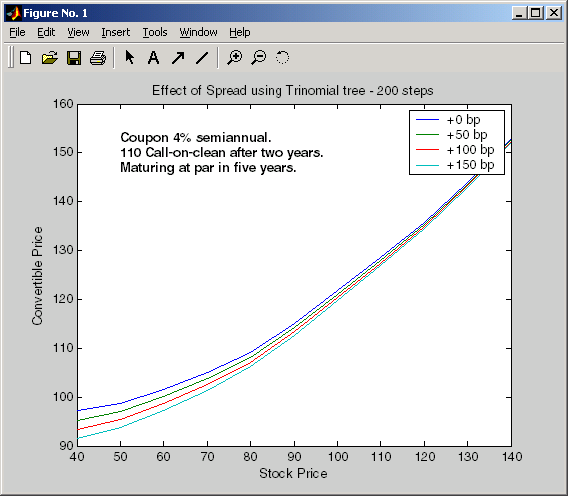
\includegraphics{figures/cbspread.png}}
\end{center}

\end{columns}
\end{frame}

\begin{frame}
Doing it in R using RQuantLib....
\vskip5pt
\scriptsize
\pagecolor{bgcolor}
\noindent
\ttfamily
\hlstd{params\ }\hlsym{$<${-}\ }\hlstd{}\hlkwc{list}\hlstd{}\hlsym{(}\hlstd{tradeDate}\hlsym{=}\hlstd{}\hlkwc{as.Date}\hlstd{}\hlsym{(}\hlstd{}\hlstr{'2002{-}01{-}02'}\hlstd{}\hlsym{),}\hspace*{\fill}\\
\hlstd{}\hlstd{\ \ \ \ \ \ \ \ \ \ \ \ \ \ \ }\hlstd{settleDate}\hlsym{=}\hlstd{}\hlkwc{as.Date}\hlstd{}\hlsym{(}\hlstd{}\hlstr{'2002{-}01{-}02'}\hlstd{}\hlsym{),}\hspace*{\fill}\\
\hlstd{}\hlstd{\ \ \ \ \ \ \ \ \ \ \ \ \ \ \ }\hlstd{}\hlkwc{dt}\hlstd{}\hlsym{=}\hlstd{}\hlnum{.25}\hlstd{}\hlsym{,}\hspace*{\fill}\\
\hlstd{}\hlstd{\ \ \ \ \ \ \ \ \ \ \ \ \ \ \ }\hlstd{interpWhat}\hlsym{=}\hlstd{}\hlstr{"discount"}\hlstd{}\hlsym{,}\hspace*{\fill}\\
\hlstd{}\hlstd{\ \ \ \ \ \ \ \ \ \ \ \ \ \ \ }\hlstd{interpHow}\hlsym{=}\hlstd{}\hlstr{"loglinear"}\hlstd{}\hlsym{)}\hspace*{\fill}\\
\hlstd{times\ }\hlsym{$<${-}\ }\hlstd{}\hlkwc{seq}\hlstd{}\hlsym{(}\hlstd{}\hlnum{0}\hlstd{}\hlsym{,}\hlstd{}\hlnum{10}\hlstd{}\hlsym{,}\hlstd{}\hlnum{.1}\hlstd{}\hlsym{)}\hspace*{\fill}\\
\hlstd{\hspace*{\fill}\\
RiskFreeRate\ }\hlsym{$<${-}\ }\hlstd{DiscountCurve}\hlsym{(}\hlstd{params}\hlsym{,\ }\hlstd{}\hlkwc{list}\hlstd{}\hlsym{(}\hlstd{flat}\hlsym{=}\hlstd{}\hlnum{0.05}\hlstd{}\hlsym{),}\hspace*{\fill}\\
\hlstd{}\hlstd{\ \ \ \ \ \ \ \ \ \ \ \ \ \ \ \ \ \ \ \ \ \ \ \ \ \ \ \ \ \ }\hlstd{times}\hlsym{)}\hspace*{\fill}\\
\hlstd{Sigma\ }\hlsym{$<${-}\ }\hlstd{}\hlnum{0.3}\hspace*{\fill}\\
\hlstd{ConvRatio\ }\hlsym{$<${-}\ }\hlstd{}\hlnum{1}\hspace*{\fill}\\
\hlstd{issueDate\ }\hlsym{$<${-}\ }\hlstd{}\hlkwc{as.Date}\hlstd{}\hlsym{(}\hlstd{}\hlstr{'2002{-}01{-}02'}\hlstd{}\hlsym{)}\hspace*{\fill}\\
\hlstd{settleDate\ }\hlsym{$<${-}\ }\hlstd{}\hlkwc{as.Date}\hlstd{}\hlsym{(}\hlstd{}\hlstr{'2002{-}01{-}02'}\hlstd{}\hlsym{)}\hspace*{\fill}\\
\hlstd{maturityDate\ }\hlsym{$<${-}\ }\hlstd{}\hlkwc{as.Date}\hlstd{}\hlsym{(}\hlstd{}\hlstr{'2007{-}01{-}02'}\hlstd{}\hlsym{)}\hspace*{\fill}\\
\hlstd{dividendYield\ }\hlsym{$<${-}\ }\hlstd{DiscountCurve}\hlsym{(}\hlstd{params}\hlsym{,\ }\hlstd{}\hlkwc{list}\hlstd{}\hlsym{(}\hlstd{flat}\hlsym{=}\hlstd{}\hlnum{0.01}\hlstd{}\hlsym{),}\hspace*{\fill}\\
\hlstd{}\hlstd{\ \ \ \ \ \ \ \ \ \ \ \ \ \ \ \ \ \ \ \ \ \ \ \ \ \ \ \ \ \ \ }\hlstd{times}\hlsym{)}\hspace*{\fill}\\
\hlstd{dividendSchedule\ }\hlsym{$<${-}\ }\hlstd{}\hlkwc{data.frame}\hlstd{}\hlsym{(}\hlstd{Type}\hlsym{=}\hlstd{}\hlkwc{character}\hlstd{}\hlsym{(}\hlstd{}\hlnum{0}\hlstd{}\hlsym{),}\hspace*{\fill}\\
\hlstd{}\hlstd{\ \ \ \ \ \ \ \ \ \ \ \ \ \ \ \ \ \ \ \ \ \ \ \ \ \ \ \ \ \ \ }\hlstd{Amount}\hlsym{=}\hlstd{}\hlkwc{numeric}\hlstd{}\hlsym{(}\hlstd{}\hlnum{0}\hlstd{}\hlsym{),}\hspace*{\fill}\\
\hlstd{}\hlstd{\ \ \ \ \ \ \ \ \ \ \ \ \ \ \ \ \ \ \ \ \ \ \ \ \ \ \ \ \ \ \ }\hlstd{Rate}\hlsym{=}\hlstd{}\hlkwc{numeric}\hlstd{}\hlsym{(}\hlstd{}\hlnum{0}\hlstd{}\hlsym{),}\hspace*{\fill}\\
\hlstd{}\hlstd{\ \ \ \ \ \ \ \ \ \ \ \ \ \ \ \ \ \ \ \ \ \ \ \ \ \ \ \ \ \ \ }\hlstd{Date}\hlsym{=}\hlstd{}\hlkwc{as.Date}\hlstd{}\hlsym{(}\hlstd{}\hlkwc{character}\hlstd{}\hlsym{(}\hlstd{}\hlnum{0}\hlstd{}\hlsym{)))}\hspace*{\fill}\\
\hlstd{callabilitySchedule\ }\hlsym{$<${-}\ }\hlstd{}\hlkwc{data.frame}\hlstd{}\hlsym{(}\hlstd{Price}\hlsym{=}\hlstd{}\hlnum{110}\hlstd{}\hlsym{,\ }\hlstd{Type}\hlsym{=}\hlstd{}\hlnum{0}\hlstd{}\hlsym{,}\hspace*{\fill}\\
\hlstd{}\hlstd{\ \ \ \ \ \ \ \ \ \ \ \ \ \ \ \ \ \ \ \ \ \ \ \ \ \ \ \ \ \ \ \ \ \ }\hlstd{Date}\hlsym{=}\hlstd{}\hlkwc{as.Date}\hlstd{}\hlsym{(}\hlstd{}\hlstr{'2004{-}01{-}02'}\hlstd{}\hlsym{))}\hspace*{\fill}\\
\hlstd{process\ }\hlsym{$<${-}\ }\hlstd{}\hlkwc{list}\hlstd{}\hlsym{(}\hlstd{underlying}\hlsym{=}\hlstd{}\hlnum{40}\hlstd{}\hlsym{,\ }\hlstd{divYield}\hlsym{=}\hlstd{dividendYield}\hlsym{,}\hspace*{\fill}\\
\hlstd{}\hlstd{\ \ \ \ \ \ \ \ \ \ \ \ \ \ \ \ }\hlstd{rff}\hlsym{=}\hlstd{RiskFreeRate}\hlsym{,\ }\hlstd{volatility}\hlsym{=}\hlstd{Sigma}\hlsym{)}\hspace*{\fill}\\
\hlstd{\hspace*{\fill}\\
bondparams\ }\hlsym{$<${-}\ }\hlstd{}\hlkwc{list}\hlstd{}\hlsym{(}\hlstd{exercise}\hlsym{=}\hlstd{}\hlstr{"eu"}\hlstd{}\hlsym{,\ }\hlstd{faceAmount}\hlsym{=}\hlstd{}\hlnum{100}\hlstd{}\hlsym{,}\hspace*{\fill}\\
\hlstd{}\hlstd{\ \ \ \ \ \ \ \ \ \ \ \ \ \ \ \ \ \ \ }\hlstd{divSch}\hlsym{=}\hlstd{dividendSchedule}\hlsym{,}\hspace*{\fill}\\
\hlstd{}\hlstd{\ \ \ \ \ \ \ \ \ \ \ \ \ \ \ \ \ \ \ }\hlstd{callSch}\hlsym{=}\hlstd{callabilitySchedule}\hlsym{,}\hspace*{\fill}\\
\hlstd{}\hlstd{\ \ \ \ \ \ \ \ \ \ \ \ \ \ \ \ \ \ \ }\hlstd{redemption}\hlsym{=}\hlstd{}\hlnum{100}\hlstd{}\hlsym{,}\hspace*{\fill}\\
\hlstd{}\hlstd{\ \ \ \ \ \ \ \ \ \ \ \ \ \ \ \ \ \ \ }\hlstd{creditSpread}\hlsym{=}\hlstd{}\hlnum{0.005}\hlstd{}\hlsym{,}\hspace*{\fill}\\
\hlstd{}\hlstd{\ \ \ \ \ \ \ \ \ \ \ \ \ \ \ \ \ \ \ }\hlstd{conversionRatio}\hlsym{=}\hlstd{ConvRatio}\hlsym{,}\hspace*{\fill}\\
\hlstd{}\hlstd{\ \ \ \ \ \ \ \ \ \ \ \ \ \ \ \ \ \ \ }\hlstd{issueDate}\hlsym{=}\hlstd{issueDate}\hlsym{,}\hspace*{\fill}\\
\hlstd{}\hlstd{\ \ \ \ \ \ \ \ \ \ \ \ \ \ \ \ \ \ \ }\hlstd{maturityDate}\hlsym{=}\hlstd{maturityDate}\hlsym{)}\hlstd{}\hspace*{\fill}\\
\mbox{}
\normalfont
\end{frame}
\begin{frame}
\scriptsize
\pagecolor{bgcolor}
\noindent
\ttfamily
\hlstd{\hspace*{\fill}\\
dateparams\ }\hlsym{$<${-}\ }\hlstd{}\hlkwc{list}\hlstd{}\hlsym{(}\hlstd{settlementDays}\hlsym{=}\hlstd{}\hlnum{3}\hlstd{}\hlsym{,}\hspace*{\fill}\\
\hlstd{}\hlstd{\ \ \ \ \ \ \ \ \ \ \ \ \ \ \ \ \ \ \ }\hlstd{dayCounter}\hlsym{=}\hlstd{}\hlstr{"Thirty360"}\hlstd{}\hlsym{,}\hspace*{\fill}\\
\hlstd{}\hlstd{\ \ \ \ \ \ \ \ \ \ \ \ \ \ \ \ \ \ \ }\hlstd{period}\hlsym{=}\hlstd{}\hlstr{"Semiannual"}\hlstd{}\hlsym{,\ }\hlstd{calendar}\hlsym{=}\hlstd{}\hlstr{"us"}\hlstd{}\hlsym{,}\hspace*{\fill}\\
\hlstd{}\hlstd{\ \ \ \ \ \ \ \ \ \ \ \ \ \ \ \ \ \ \ }\hlstd{businessDayConvention}\hlsym{=}\hlstd{}\hlstr{"Following"}\hlstd{}\hlsym{,}\hspace*{\fill}\\
\hlstd{}\hlstd{\ \ \ \ \ \ \ \ \ \ \ \ \ \ \ \ \ \ \ }\hlstd{todayDate}\hlsym{=}\hlstd{issueDate}\hlsym{)}\hspace*{\fill}\\
\hlstd{coupon\ }\hlsym{$<${-}\ }\hlstd{}\hlnum{0.04}\hspace*{\fill}\\
\hlstd{\hspace*{\fill}\\
ret\ }\hlsym{$<${-}\ }\hlstd{}\hlkwc{data.frame}\hlstd{}\hlsym{()}\hspace*{\fill}\\
\hlstd{}\hlkwa{for\ }\hlstd{}\hlsym{(}\hlstd{s\ }\hlkwa{in\ }\hlstd{}\hlkwc{c}\hlstd{}\hlsym{(}\hlstd{}\hlnum{0}\hlstd{}\hlsym{,\ }\hlstd{}\hlnum{0.005}\hlstd{}\hlsym{,\ }\hlstd{}\hlnum{0.010}\hlstd{}\hlsym{,\ }\hlstd{}\hlnum{0.015}\hlstd{}\hlsym{))\{}\hspace*{\fill}\\
\hlstd{\hspace*{\fill}\\
}\hlstd{\ \ }\hlstd{x\ }\hlsym{$<${-}\ }\hlstd{}\hlkwc{c}\hlstd{}\hlsym{()}\hspace*{\fill}\\
\hlstd{}\hlstd{\ \ }\hlstd{y\ }\hlsym{$<${-}\ }\hlstd{}\hlkwc{c}\hlstd{}\hlsym{()}\hspace*{\fill}\\
\hlstd{}\hlstd{\ \ }\hlstd{i\ }\hlsym{$<${-}\ }\hlstd{}\hlnum{1}\hspace*{\fill}\\
\hlstd{}\hlstd{\ \ }\hlstd{}\hlkwa{for\ }\hlstd{}\hlsym{(}\hlstd{p\ }\hlkwa{in\ }\hlstd{}\hlkwc{seq}\hlstd{}\hlsym{(}\hlstd{}\hlnum{0}\hlstd{}\hlsym{,\ }\hlstd{}\hlnum{100}\hlstd{}\hlsym{,\ }\hlstd{}\hlkwc{by\ }\hlstd{}\hlsym{=\ }\hlstd{}\hlnum{10}\hlstd{}\hlsym{))\ \{}\hspace*{\fill}\\
\hlstd{}\hlstd{\ \ \ \ }\hlstd{process\$underlying\ }\hlsym{$<${-}\ }\hlstd{}\hlnum{40}\hlstd{}\hlsym{+}\hlstd{p\hspace*{\fill}\\
}\hlstd{\ \ \ \ }\hlstd{bondparams\$creditSpread\ }\hlsym{$<${-}\ }\hlstd{s\hspace*{\fill}\\
}\hlstd{\ \ \ \ }\hlstd{}\hlkwc{t\ }\hlstd{}\hlsym{$<${-}\ }\hlstd{ConvertibleFixedCouponBond}\hlsym{(}\hlstd{bondparams}\hlsym{,}\hspace*{\fill}\\
\hlstd{}\hlstd{\ \ \ \ \ \ \ \ \ \ \ \ \ \ \ \ \ \ \ \ \ \ \ \ \ \ \ \ \ \ \ \ \ \ \ \ }\hlstd{coupon}\hlsym{,}\hspace*{\fill}\\
\hlstd{}\hlstd{\ \ \ \ \ \ \ \ \ \ \ \ \ \ \ \ \ \ \ \ \ \ \ \ \ \ \ \ \ \ \ \ \ \ \ \ }\hlstd{process}\hlsym{,}\hspace*{\fill}\\
\hlstd{}\hlstd{\ \ \ \ \ \ \ \ \ \ \ \ \ \ \ \ \ \ \ \ \ \ \ \ \ \ \ \ \ \ \ \ \ \ \ \ }\hlstd{dateparams}\hlsym{)}\hspace*{\fill}\\
\hlstd{}\hlstd{\ \ \ \ }\hlstd{x}\hlsym{{[}}\hlstd{i}\hlsym{{]}\ $<${-}\ }\hlstd{p\ }\hlsym{+\ }\hlstd{}\hlnum{40}\hspace*{\fill}\\
\hlstd{}\hlstd{\ \ \ \ }\hlstd{y}\hlsym{{[}}\hlstd{i}\hlsym{{]}\ $<${-}\ }\hlstd{}\hlkwc{t}\hlstd{\$cleanPrice\hspace*{\fill}\\
}\hlstd{\ \ \ \ }\hlstd{i\ }\hlsym{$<${-}\ }\hlstd{i\ }\hlsym{+\ }\hlstd{}\hlnum{1}\hspace*{\fill}\\
\hlstd{}\hlstd{\ \ }\hlstd{}\hlsym{\}}\hspace*{\fill}\\
\hlstd{}\hlstd{\ \ }\hlstd{z\ }\hlsym{$<${-}\ }\hlstd{}\hlkwc{rep}\hlstd{}\hlsym{(}\hlstd{s}\hlsym{,\ }\hlstd{}\hlnum{11}\hlstd{}\hlsym{)}\hspace*{\fill}\\
\hlstd{}\hlstd{\ \ }\hlstd{ret\ }\hlsym{$<${-}\ }\hlstd{}\hlkwc{rbind}\hlstd{}\hlsym{(}\hlstd{ret}\hlsym{,\ }\hlstd{}\hlkwc{data.frame}\hlstd{}\hlsym{(}\hlstd{Stock}\hlsym{=}\hlstd{x}\hlsym{,}\hlstd{ConvPrice}\hlsym{=}\hlstd{y}\hlsym{,}\hlstd{z}\hlsym{))}\hspace*{\fill}\\
\hlstd{}\hlsym{\}}\hspace*{\fill}\\

\hlstd{}\hspace*{\fill}\\
\hspace*{\fill}\\
\hspace*{\fill}\\
\mbox{}
\normalfont
\end{frame}

\begin{frame}
\vskip10pt
\scriptsize
\pagecolor{bgcolor}
\noindent
\ttfamily
\hlstd{}\hlkwc{>library}\hlstd{}\hlsym{(}\hlstd{ggplot2}\hlsym{)}\hspace*{\fill}\\
\hlstd{>p\ }\hlsym{$<${-}\ }\hlstd{ggplot}\hlsym{(}\hlstd{ret}\hlsym{,\ }\hlstd{aes}\hlsym{(}\hlstd{Stock}\hlsym{,}\hlstd{ConvPrice}\hlsym{,\ }\hlstd{colour}\hlsym{=}\hlstd{}\hlkwc{factor}\hlstd{}\hlsym{(}\hlstd{z}\hlsym{)))}\hspace*{\fill}\\
\hlstd{>p\ }\hlsym{+\ }\hlstd{geom\textunderscore line}\hlsym{()\ +\ }\hlstd{scale\textunderscore colour\textunderscore discrete}\hlsym{(}\hlstd{}\hlstr{"Spread"}\hlstd{}\hlsym{)}\hspace*{\fill}\\
\hlstd{}\hlsym{+\ }\hlstd{opts}\hlsym{(}\hlstd{}\hlkwc{title}\hlstd{}\hlsym{=}\hlstd{}\hlstr{'Effect\ of\ spread\ on\ a\ convertible\ bond'}
\normalfont
\begin{center}
\resizebox{75mm}{!}{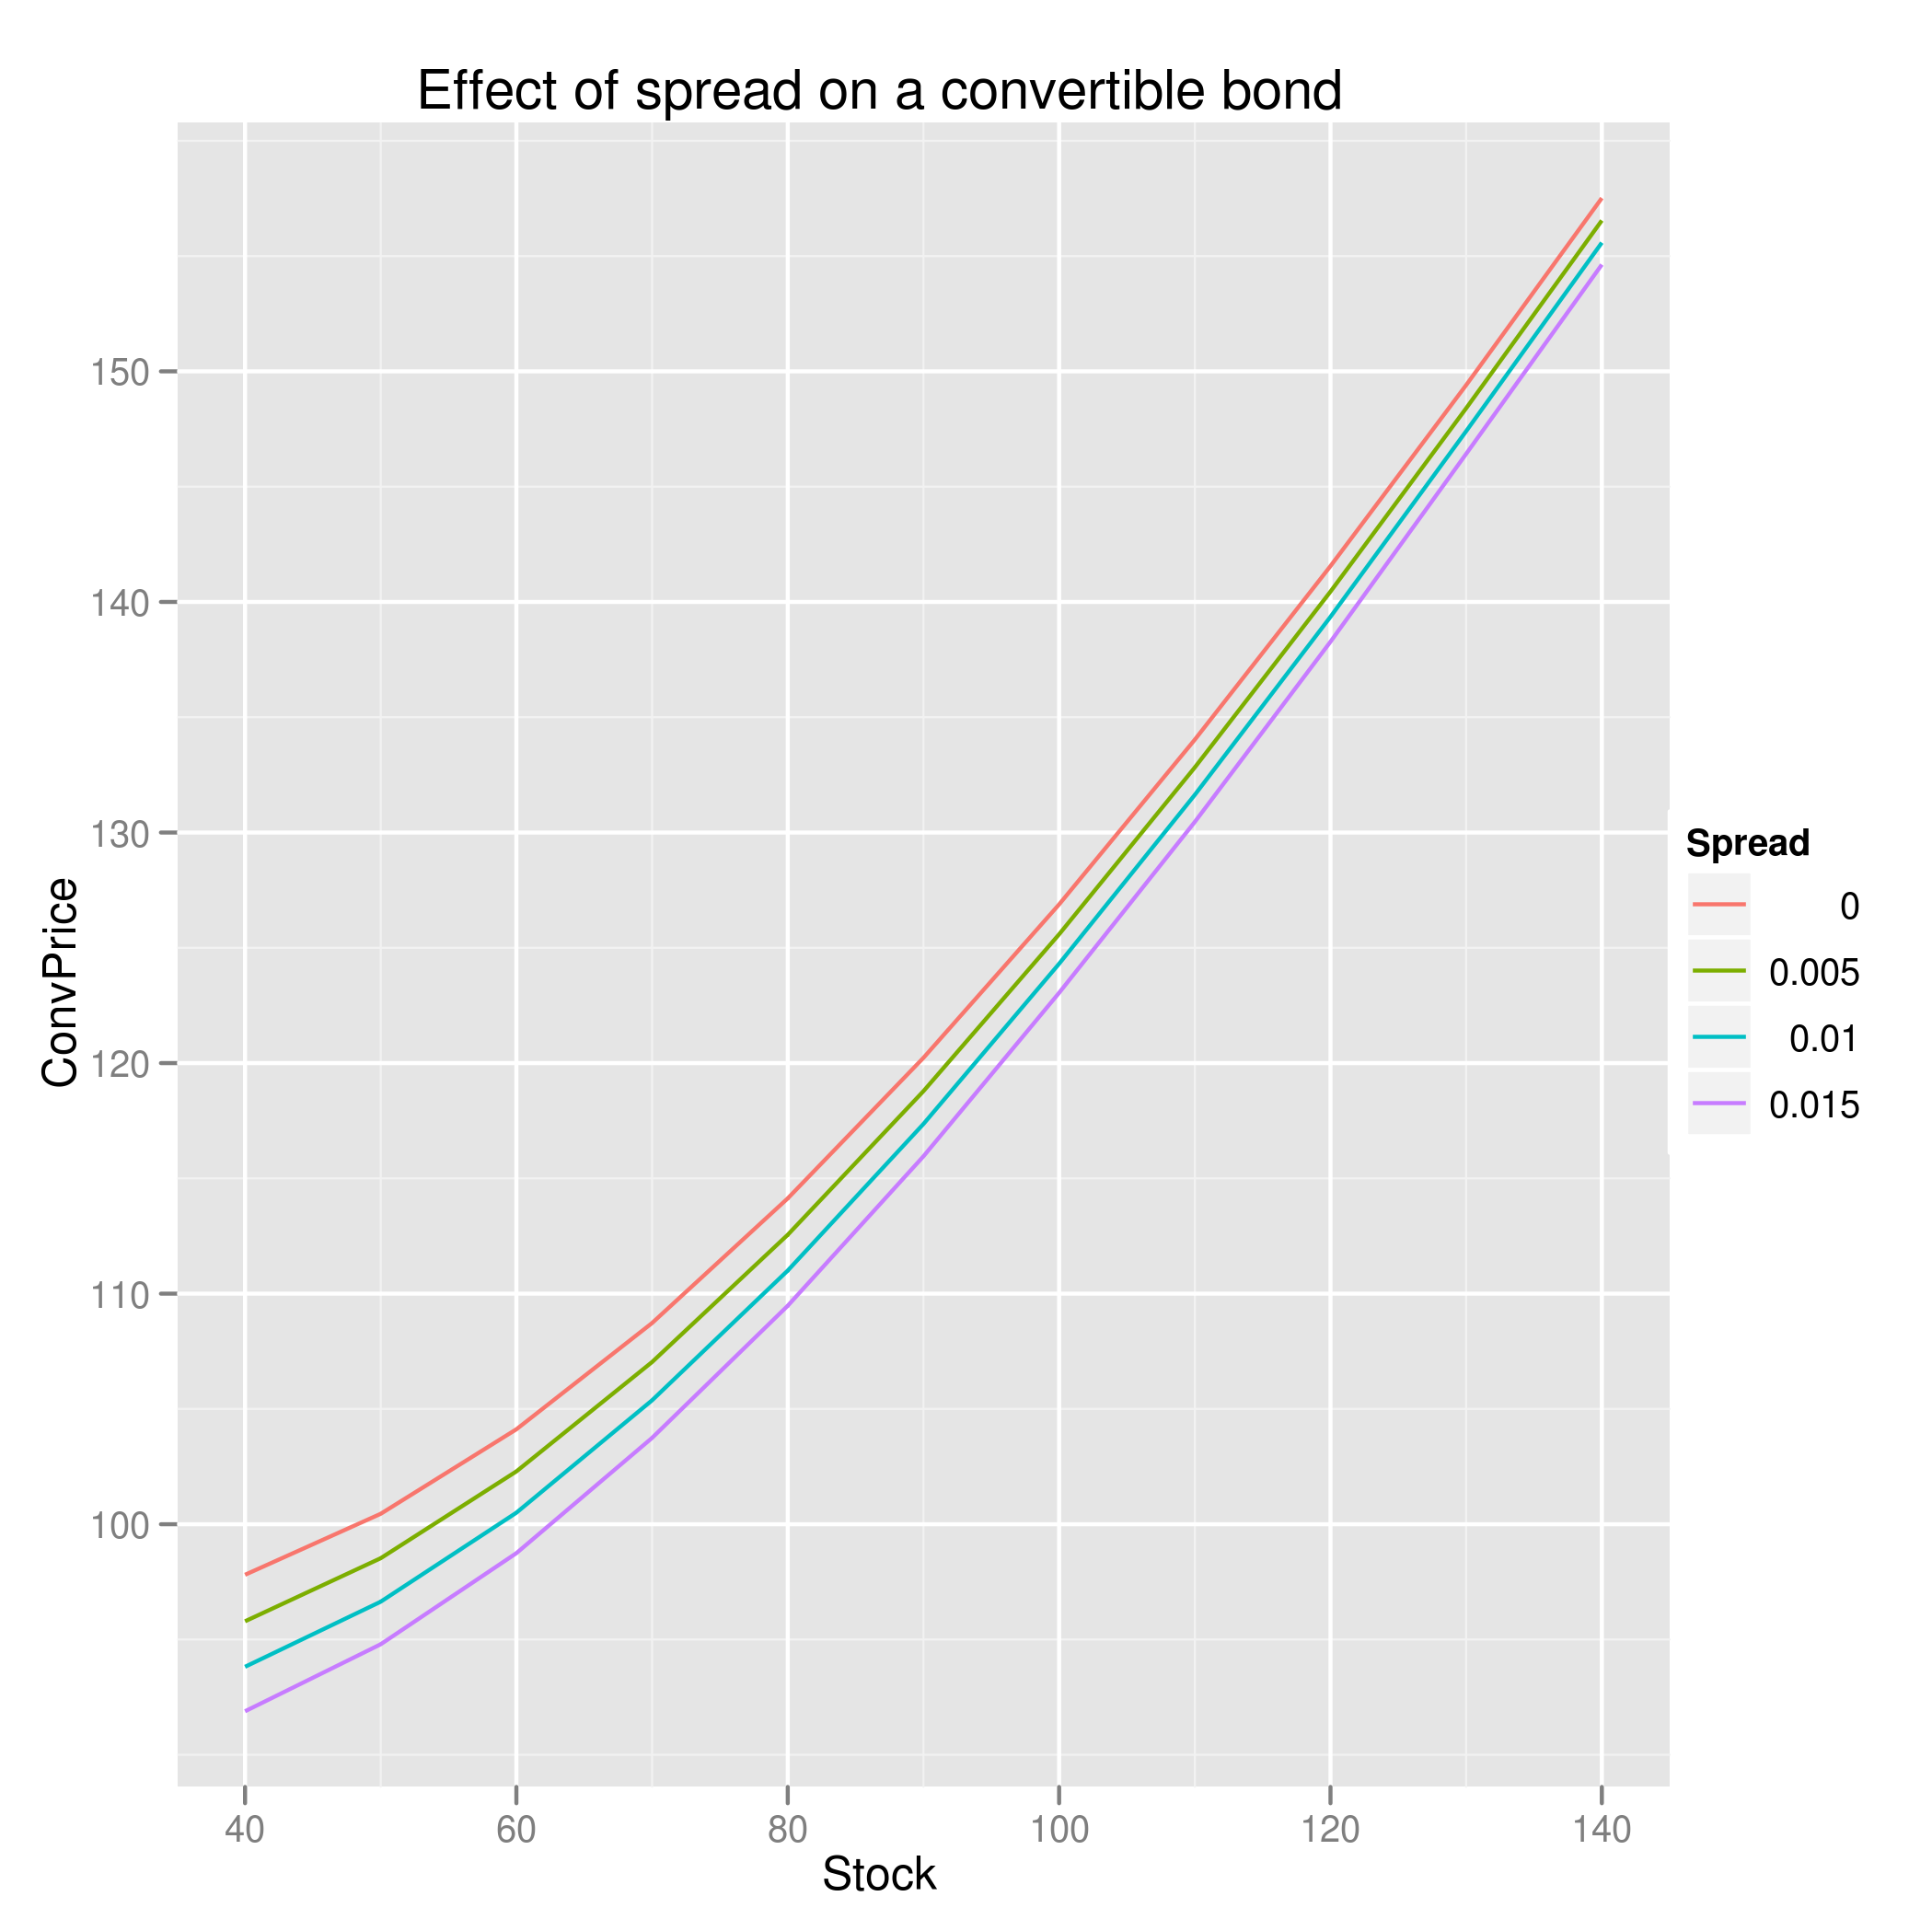
\includegraphics{figures/matlab_cbond.png}}
\end{center}
\end{frame}

\begin{frame}
	\frametitle{Fixed Income in RQuantLib}
	\framesubtitle{Graphical User Interface}		
RQuantLib also comes with an user interface via the 'traitr' package by professor John Verzani.
\begin{center}
	\resizebox{90mm}{!}{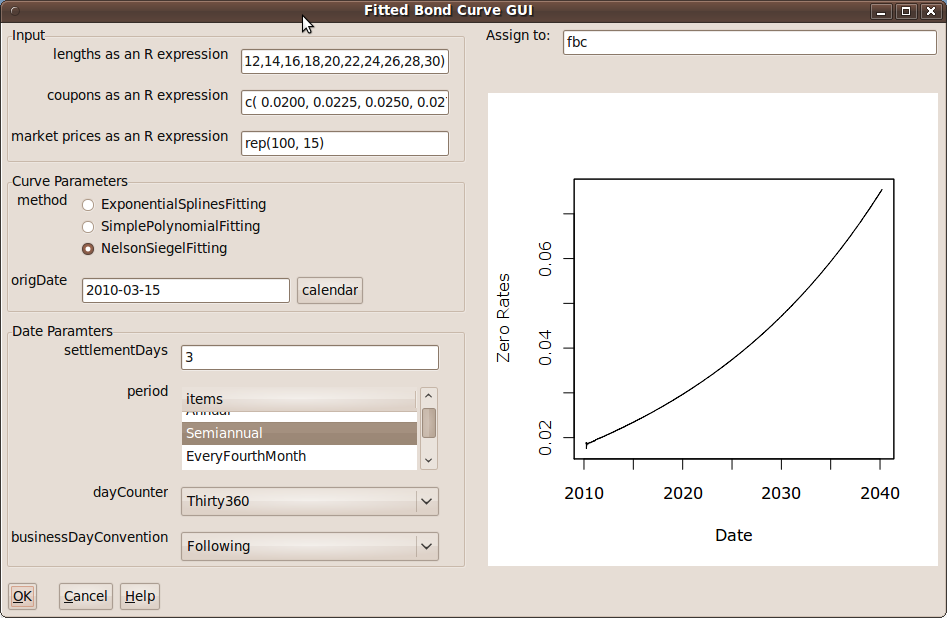
\includegraphics{figures/fbGUI.png}}
\end{center}
\end{frame}

\begin{frame}
	\frametitle{Fixed Income in RQuantLib}
	\framesubtitle{Graphical User Interface}	
\begin{center}
	\resizebox{110mm}{!}{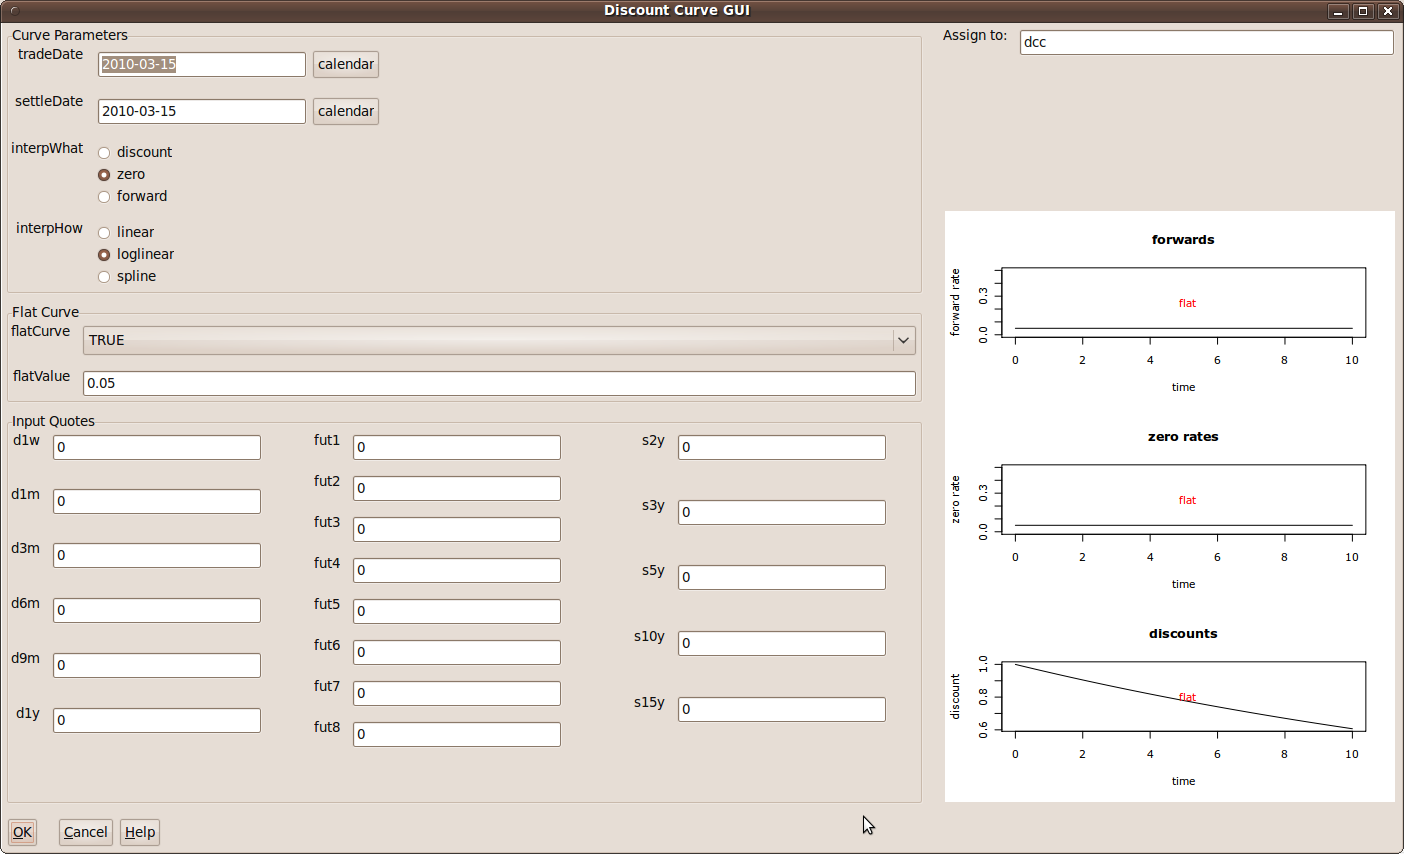
\includegraphics{figures/dcGUI.png}}
\end{center}
\end{frame}


\begin{frame}
	\frametitle{Fixed Income in RQuantLib}
	\framesubtitle{Graphical User Interface}		
\begin{center}
	\resizebox{90mm}{!}{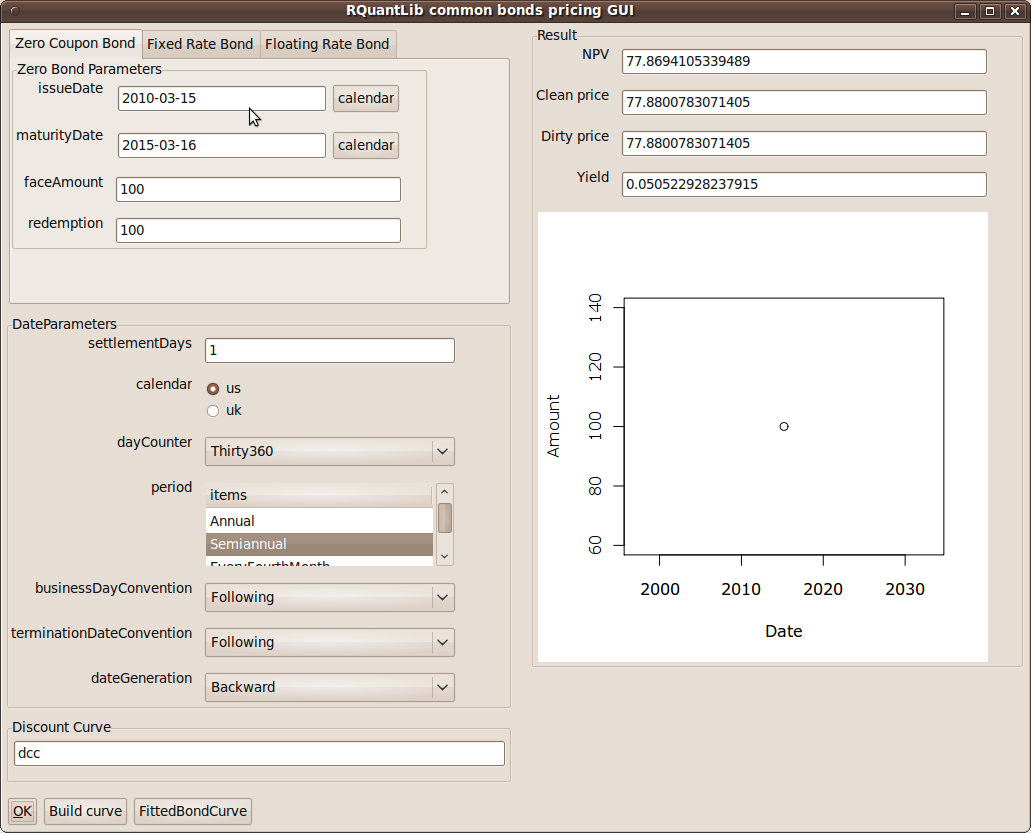
\includegraphics{figures/bondGUI.png}}
\end{center}
\end{frame}



\end{document}

%%% Local Variables: 
%%% mode: latex
%%% TeX-master: t
%%% End: 
